\chapter{General Theory}

%\section{Introduction}
It is now widely accepted that many of the advances in modern continuum mechanics are largely due to the clear distinction — made, in fact, not very long ago — between the fundamental components that form its structure: \textit{kinematics}, the \textit{balance} laws, and the \textit{constitutive} characterization of material response. These pertain to three foundational substructures upon which mechanics is built: the definition of the \textit{bodies} under investigation,\footnote{Answering questions such as what a body is in continuum physics, how one may define a part of it, or what structure the points composing the body possess — however seemingly trivial — actually requires a careful investigation of both mathematical and epistemological nature.} a geometry along with its associated \textit{kinematics}, and a theory of \textit{forces}.

The relationships among the placements of bodies, their shape, forces, and time can be of different kinds: general, such as those governing \textit{statics} — which examines putative equilibria — and \textit{dynamics} — which describes motion; or particular, namely the \textit{constitutive} relations, which define a material.

This chapter is devoted to the study of kinematics, the first pillar of the theory. We shall introduce the basic geometric notions necessary to describe bodies, their configurations in space, and their admissible motions. Emphasis will be placed on the abstract structure underlying these concepts, with the aim of providing a clear and general framework that can accommodate both classical and more advanced formulations of continuum mechanics.


\section{Deformation}
We   identify a \textit{body} $\Bc$ as a manifold of \textit{material points}, denoted by $X$. We assume that these points are primitive elements of Mechanics, in the same way that numbers are in Analysis.

We assume that a body can occupy various regions of ambient space,\footnote{Quoting Clifford Truesdell: ``Bodies are available to us only in their configurations, the regions they happen
	to occupy in Euclidean space at some time''.} which we  identify with the three-dimensional Euclidean space $\Ec$. We denote by $\Vc$ the associated vector space of translations.


We observe bodies against the framework of this spatial structure, a background that plays the role of the wall observed by the prisoners in Plato's cave. Unlike those prisoners, we are not interested in breaking our chains and running out to experience the ``real'' world, only to return to the cave and compare the shadows on the wall with their ``true'' counterparts. We simply do not consider ourselves prisoners and are instead concerned with providing a mathematical model of our only given experience, those shadows.

\begin{figure}[h!]
	\centering
	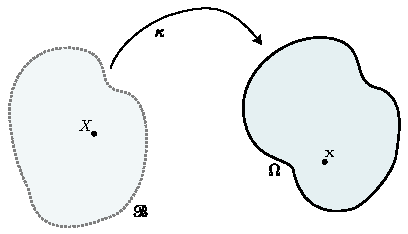
\includegraphics[scale=1.2]{figure/cinematica/piazzamento3d}
	\caption{Placement $\kappa$.}
	\label{fig:piazzamento3d}
\end{figure}
The manifold $\Bc$ is generally assumed to be regular, that is, a diffeomorphism of a domain in Euclidean space. Specifically, we state that an open set $\Omega$ in $\Ec$ is occupied by the body $\Bc$ if there exists an \textit{injective} function, called a \textit{placement} or \textit{configuration}, that maps $\Bc$ into $\Omega$:
\begin{equation}
	\kappa\,:\,\Bc\to \Omega\in \Ec.
\end{equation}
The placement $\kappa$ thus maps the material points $X$ into elements $\xb$ of the three-dimensional vector space $\Vc$; $\xb$ is therefore the position occupied by the point $X$ in the placement $\kappa$. Somewhat imprecisely, we will call $\xb$ a ``point'', meaning the position occupied by $\kappa(X)$. Similarly, we will write $\xb\in \Omega$, imagining identifying $\Omega=\fb(\Bc)$ with the set of positions of its points.

The injectivity of placements ensures that each point in Euclidean space corresponds to at most one material point. This assumption prevents the so-called ``interpenetration of matter.'' Moreover, we shall assume that placements are \textit{surjective}, meaning that for every point $\Bc$ in the set $\Omega$, there exists at least one point $\kappa(\Bc)$; in other words, the placement does not generate new points.

It follows that the placement $\kappa$ is a \textit{bijective} map and therefore admits an inverse
\begin{equation}
	\kappa^{-1}\,:\,\kappa(\Bc)=\Omega\mapsto\Bc.
\end{equation}



If $\chi$ is another placement, we can define the function
\begin{equation}
	\fb\,:\, \kappa(\Bc)\mapsto\chi(\Bc)
\end{equation}
as $\fb\coloneqq\chi\circ \kappa^{-1}$. This function is the \textit{deformation} from configuration $\kappa$ to configuration $\chi$. We observe that  $\fb$ is a vector field. Thus, if $\xb=\kappa(X)$, we say that $\xb$ and $\fb(\xb)$ are the positions occupied by the material point $X$ before and after the deformation $\fb$, respectively.

We can choose once and for all a configuration, called \textit{reference} configuration, and distinguish a second one as \textit{current}. 	When necessary, we will also distinguish $\Ecu$, $\Er$, and  $\Vcu$ $\Vr$ for the current and referential copies of $\Ec$ and $\Vc$.

\begin{figure}[h]
	\centering
	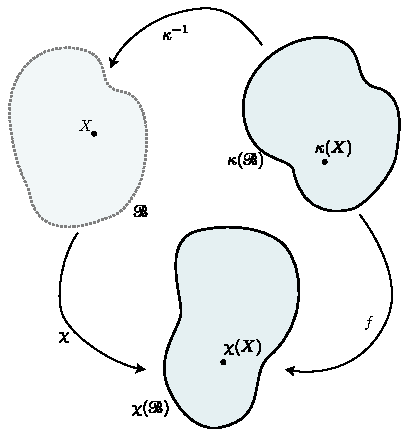
\includegraphics[scale=1.2]{figure/cinematica/def3d}
	\caption{Deformation $f$.}
	\label{fig:def3d}
\end{figure}



\subsection{Deformation Gradient}  
We assume that $\fb$ and $\fb^{-1}$ are continuous and differentiable. This circumstance avoids some pathological situations, that may occur in fracture mechanics, thal we will not consider. To infer the local effect of the deformation, we need to explore a neighborhood in a certain direction $\hb\in \Vc$, whose length $|\hb|$ will be made to tend to zero. This operation defines the directional derivative of $\fb$, which can be expressed in terms of the \textit{deformation gradient} $\partial_\xb \fb=\nabla\fb\equiv\Fb$ according to the following definition; let $\hb =\varepsilon \eb$, where $\eb$ is a unit vector and $\varepsilon=|\hb|$, we have

\begin{definition}  
	\begin{equation}  
		\lim_{\varepsilon\to0}\frac{\fb(\xb+\varepsilon \eb)-\fb(\xb)}{\varepsilon}=:\Fb(\xb)\eb.  
	\end{equation}  
\end{definition}  

This relation can be easily rewritten as  
\begin{equation}  
	\fb(\xb+\hb)-\fb(\xb)=\Fb(\xb)\hb+o(|\hb|).  
\end{equation}  
Thus, up to higher-order infinitesimals compared to $|\hb|$, the vector $\xb+\hb-\xb=\hb$ is mapped to $\Fb(\xb)\hb$.  

If $\{\eb_i\}$ is a Cartesian basis, then the deformation gradient can be written as  
\begin{equation}  
	\Fb=\fb,_{i}\otimes\eb_i.  
\end{equation}  

We require  that  
\begin{equation}\label{detpos}  
	\det \Fb(\xb)>0 \qquad\forall \xb\in\Omega.  
\end{equation}  

The physical interpretation of \eqref{detpos} is easily understood by recalling the definition of the determinant of a second-order tensor $\Ab\in\Lin$: given three non-collinear vectors $\ub, \vb,\wb\in \Vc$, the determinant of $\Ab$ is the number  
\begin{equation}\label{det}  
	\det \Ab\coloneqq \frac{\Ab\ub\times\Ab\vb\cdot\Ab\wb}{\ub\times\vb\cdot\wb}.  
\end{equation}  
The denominator on the right-hand side of \eqref{det} is the signed volume (positive if the triplet $\ub, \vb,\wb$ is positively oriented) of the parallelepiped spanned by $\ub, \vb,\wb$, while the numerator represents the signed volume of the parallelepiped spanned by $\Ab\ub, \Ab\vb,\Ab\wb$, that is, the images of the original vectors under the mapping $\Ab$. In particular, if $\Ab=\Fb$, the numerator represents the volume of the deformed parallelepiped under $\fb$. Thus, if $\det \Fb(\xb)$ were zero, it would mean that the original parallelepiped has collapsed into a point, which we want to avoid; furthermore, if it were negative, it would mean that the orientation of the original triplet has changed, which we also wish to prevent.  

Let us now explicitly write the components of the deformation gradient. By definition, we have:  
\begin{equation}  
	\begin{aligned}  
		F_{ij}=(\Fb\eb_j)\cdot \eb_i=\fb_{,j}\cdot \eb_i=f_{i,j}.  
	\end{aligned}  
\end{equation}  
The matrix representing $\Fb$ in the basis $\{\eb_i\}$ is then  
\begin{equation}  
	[\Fb]=  
	\begin{bmatrix}  
		f_{1,1}&f_{1,2}&f_{1,3}\\f_{2,1}&f_{2,2}&f_{2,3}\\f_{3,1}&f_{3,2}&f_{3,3}  
	\end{bmatrix}.  
\end{equation}  


\begin{remark}
	In order to study the deformation of $\Bc$, we can introduce two copies of the pair $(\Ec,\Vc)$, the referential pair $(\Er, \Vr)$ and the current pair $(\Ecu, \Vcu)$.
	A deformation is a map $\fb:\xb\mapsto \yb=\fb(\xb)$ from $\Er$ to $\Ecu$.  The deformation gradient $\Fb$ maps vector of $\Vr$ into $\Vcu$. Then $\Fb$ is not properly a second order tensor, since it is not a map of a space into itself; for this reason it is sometimes called \textit{double vector} or \textit{two-point tensor}.
\end{remark}

\begin{exercise}  
	Given the deformation $\fb(\xb)=\xb+\alpha x_2\eb_2+\beta x_2x_3\eb_3$, with $\xb=x_1\eb_1+x_2\eb_2+x_3\eb_3$. Determine the deformation gradient.  
	\begin{svolgimento}  
		The components of the deformation are:  
		\begin{equation}  
			\begin{aligned}  
				&f_{1}=\fb\cdot \eb_{1}=x_{1},\\  
				&f_{2}=\fb\cdot \eb_{2}=x_{2}+\alpha x_{2},\\  
				&f_{3}=\fb\cdot \eb_{3}=x_{3}+\beta x_{2}x_{3},  
			\end{aligned}  
		\end{equation}  
		from which we immediately obtain  
		\begin{equation}  
			[\Fb]=  
			\begin{bmatrix}  
				f_{1,1}&f_{1,2}&f_{1,3}\\f_{2,1}&f_{2,2}&f_{2,3}\\f_{3,1}&f_{3,2}&f_{3,3}  
			\end{bmatrix}=  
			\begin{bmatrix}  
				1&0&0\\0&1+\alpha&0\\0&\beta x_3&1+\beta x_2  
			\end{bmatrix}.  
		\end{equation}  
		Without resorting to the matrix representation, we can immediately write:  
		\begin{equation}  
			\Fb=\fb_{,i}\otimes\eb_i=\eb_1\otimes\eb_1+(1+\alpha)\eb_2\otimes\eb_2+\beta x_3\eb_3\otimes\eb_2+(1+\beta x_2)\eb_3\otimes\eb_3.  
		\end{equation}  
	\end{svolgimento}  
\end{exercise}  


\subsection{Displacement}  
If $\xb$ and $\fb(\xb)$ are, respectively, the positions occupied by a material point in two placements, their difference defines the displacement vector:  
\begin{definition}  
	\begin{equation}  
		\ub(\xb)\coloneqq\fb(\xb)-\xb.  
	\end{equation}  
\end{definition}  

\begin{figure}  
	\centering  
	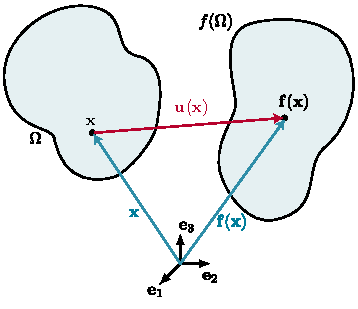
\includegraphics[scale=1.2]{figure/cinematica/displ}  
	\caption{Displacement vector.}  
	\label{fig:displ}  
\end{figure}  

Its gradient, which we denote by $\Hb\coloneqq\nabla\ub$, is given by  

\begin{definition}  
	\begin{equation}\label{HFI}  
		\Hb(\xb)=\Fb(\xb)-\Ib,  
	\end{equation}  
\end{definition}  
where $\Ib$ is the identity tensor. If $\{\eb_i\}$ is a Cartesian basis, then  
\begin{equation}  
	\Hb=\ub,_i\otimes\eb_i  
\end{equation}  
and the components of $\Hb$ are immediately obtained as  
\begin{equation}  
	H_{ij}=\Hb\eb_j\cdot\eb_i=u_{i,j}.  
\end{equation}  

\begin{remark}
The condition \eqref{detpos}   becomes particularly clear in a one-dimensional context. Let us therefore consider a continuum embedded in a one-dimensional Euclidean space, aligned with the direction $\eb$. A point is then given by $\xb = x\eb$, the deformation by $\fb(x) = f(x)\eb$, and the displacement by $\ub(x) = u(x)\eb = (f(x) - x)\eb$. In this elementary setting, condition \eqref{detpos}   translates into the requirement that $f'>0$, that is, the deformation must be monotonically increasing.

Let $L$ denote the length of the domain $\Omega$, whose endpoints we label as points $A$ and $B$; the assumption of monotonicity for the deformation becomes the condition
\begin{equation}
	u'(x) > -1,
\end{equation}
which, when integrated over $\Omega$, yields the inequality
\begin{equation}
	u(L) > u(0) - L.
\end{equation}
If this inequality were not satisfied, then after the deformation point $B$ could end up to the left of point $A$. In other words, the oriented segment $\big( x(B)-x(A) \big)\eb$, which in the undeformed configuration pointed from $A$ to $B$ along the direction $\eb$, could be deformed into a segment oriented in the opposite direction, leading to interpenetration of matter.

\begin{center}
	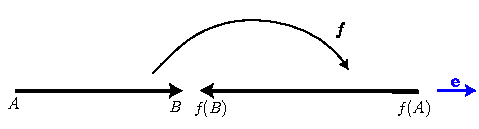
\includegraphics[scale=1.3]{figure/cinematica/orient1d}
\end{center}

We therefore say that the condition $f'(x) > 0$ ensures the preservation of spatial orientation (segments initially oriented along $\eb$ remain so) and the prevention of interpenetration of matter. Finally, observe that the inequality must be strict: if we had $u(L) - u(0) = -L$, the endpoints of the segment would collapse into a single point—an outcome we seek to avoid.
\end{remark}

\section{Change in Length}  
Let us consider, in a reference configuration, two 'nearby' points $\xb$ and $\xb_0$. The infinitesimal segment they define has a length  
\begin{equation}  
	d\ell_0=|\xb-\xb_0|.  
\end{equation}  
Denoting by $\tb$ the unit vector that defines the direction,  
\begin{equation}  
	\tb\coloneqq\frac{\xb-\xb_0}{|\xb-\xb_0|},  
\end{equation}  
we can write  
\begin{equation}  
	\xb-\xb_0=d\ell_0 \tb.  
\end{equation}  
The images of $\xb$ and $\xb_0$ under the deformation are $\fb(\xb)$ and $\fb(\xb_0)$, which define a segment of length  
\begin{equation}  
	d\ell:=|\mathbf{f}(\mathbf{x})-\mathbf{f}(\mathbf{x}_0)|.  
\end{equation}  

\begin{center}  
	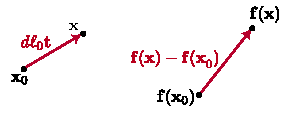
\includegraphics[scale=1.2]{figure/cinematica/dl}  
\end{center}  

Expanding the deformation in a Taylor series around $\xb_0$, we have  
\begin{equation}  
	\mathbf{f}(\mathbf{x})=\mathbf{f}(\mathbf{x}_{0})+\mathbf{F}(\mathbf{x}_{0})[\mathbf{x-x}_{0}]+o(|\mathbf{x-x}_{0}|),  
\end{equation}  
or equivalently,  
\begin{equation}  
	\mathbf{f}(\mathbf{x})-\mathbf{f}(\mathbf{x}_0)=d\ell_0\mathbf{F}\mathbf{t}+o(d\ell_0),  
\end{equation}  
from which it follows that  
\begin{equation}  
	d\ell=|\mathbf{f}(\mathbf{x})-\mathbf{f}(\mathbf{x}_0)|=d\ell_0|\mathbf{F}\mathbf{t}|+o(d\ell_0).  
\end{equation}  
Thus, up to higher-order infinitesimals of order $o(d\ell_0)$, the ratio between the two lengths is given by  
\begin{definition}  
	\begin{equation}\label{dl}  
		\frac{d\ell}{d\ell_0}=|\mathbf{Ft}|.  
	\end{equation}  
\end{definition}  

We have therefore concluded that, given an infinitesimal segment in the direction $\tb$ in the reference configuration, the ratio between the length of the deformed segment and the length of the undeformed segment equals the norm of the deformation gradient applied to $\tb$.  

Observe that $|\mathbf{Ft}|$ can be rewritten as  
\begin{equation}  
	|\mathbf{Ft}|=\sqrt{\Fb\tb\cdot\Fb\tb}=\sqrt{\Fb^\top\Fb\tb\cdot\tb}.  
\end{equation}  
Introducing the \textit{right Cauchy-Green tensor},  
\begin{definition}  
	\begin{equation}  
		\Cb\coloneqq\Fb^\top\Fb,  
	\end{equation}  
\end{definition}  
the ratio between the deformed and undeformed segment lengths can alternatively be written as  
\begin{equation}  
	\frac{d\ell}{d\ell_0}=\sqrt{\Cb\tb\cdot\tb}.  
\end{equation}  

\begin{remark}  
	It is interesting to note that $\Cb^\top=(\Fb^\top\Fb)^\top=\Fb^\top\Fb=\Cb$, so $\Cb$ is symmetric. This observation suggests that, to evaluate length variations, it is not necessary to know the entire deformation gradient $\Fb$, which generally has nine components. It is sufficient to know $\Cb$, which is characterized by six components. This implies that the deformation gradient $\Fb$ contains more information than $\Cb$, but this additional information is not required to describe length variations. It is not difficult to infer that the extra information concerns the rigid component of the deformation, as we will see later.  
\end{remark}  



\section{Change in Area}



Let us now consider  three non collinear points $\xb_0$, $\xb_0+\ab$, $\xb_0+\bb$ in the reference configuration, $\ab$, $\bb$ infinitesimal.
The vectors $\ab$ and $\bb$ define the oriented surface whose normal is
\begin{equation}
	\nb_{\rm ref}=\frac{\ab\times\bb}{|\ab\times\bb|};
\end{equation}
 the quantity
\begin{equation}
	da_0=|\ab\times\bb|
\end{equation}
 is a measure of the area of the oriented surface. In the deformed configuration, the area of the deformed surface is
 \begin{equation}
 da=|\Fb \ab \times \Fb \bb|
 \end{equation}
 and the deformed normal vector is 
 \begin{equation}
 \nb_{\rm cur}=\frac{\Fb \ab \times \Fb \bb}{|\Fb \ab \times \Fb \bb|}.
 \end{equation}
 We need to relate $ \nb_{\rm ref}$ and $ \nb_{\rm cur}$
 
To do this, we need some algebra. In particular, we recall that the determinant is an operator that assigns to each second order tensor $\Ab$ a scalar $\det\Ab$ defined by
\begin{equation}\label{det}
	\det\Ab=\frac{\Ab\ub\cdot(\Ab\vb\times \Ab\wb)}{\ub\cdot(\vb\times \wb)},
\end{equation}
for any basis $\{\ub,\vb,\wb\}$. It is easy to see then that $|\det\Ab|$ is the ratio of the volume of the parallelepiped defined by the vectors $\Ab\ub$, $\Ab\vb$ and $\Ab\wb$ to the volume of the parallelepiped defined by the vectors $\{\ub,\vb,\wb\}$. 

Now let $\Ab$ invertible and let define $\bar\ub=\Ab \ub$; therefore the following equality holds for all $\bar{\ub}$:
\begin{equation}
\bar{\ub} \cdot( \Ab \vb\times\Ab\wb)=(\det\Ab)\Ab^{-1} \bar{\ub}\cdot (\vb\times\wb)=(\det\Ab)\bar{\ub}\cdot\Ab^{-\top}(\vb\times\wb),
\end{equation}
 whence we deduce that
%
%
%
%Now, let
%\begin{equation}
%	\ab:=\Ab \ub\times\Ab \vb;
%\end{equation}
%since $\Ab\ub\cdot \ab=\Ab\vb\cdot\ab=0$, it follows that $\Ab^\top\ab$ is orthogonal to $\ub$ and $\vb$ and then there exist $\gamma\in\Ro$ such that
%\begin{equation}
%	\Ab^\top\ab=\gamma(\ub\times\vb) \quad \Longrightarrow \quad\Ab^\top(\Ab\ub\times\Ab\vb)=\gamma(\ub\times\vb).
%\end{equation}
%Let $\wb=\ub\times\vb$; then
%\begin{equation}
%	\gamma\wb\cdot(\ub\times\vb)=\wb\cdot\Ab^\top(\Ab\ub\times\Ab\vb)=\Ab\wb\cdot (\Ab\ub\times\Ab\vb).
%\end{equation}
%This latter relation reveals that $\gamma=\det\Ab$ and then
%\begin{equation}
%	\Ab^\top(\Ab\ub\times\Ab\vb)=\det\Ab(\ub\times\vb),
%\end{equation}
%or rather
\begin{equation}\label{cofactor}
	\Ab \vb\times \Ab \wb =\Ab^*(\vb\times\wb), \quad \Ab^*:=(\det\Ab)\Ab{^{-\top}}.
\end{equation}
The tensor $\Ab^*$ is the cofactor of $\Ab$. With \eqref{cofactor}, the current normal vector becomes
\begin{equation}
	\nb_{\rm cur}=\frac{\Fb\ab\times\Fb\ab}{|\Fb\ab\times\Fb\ab|}=\frac{\Fb^*\nb_{\rm ref}}{|\Fb^*\nb_{\rm ref}|},
\end{equation}
whence we deduce the
\begin{definition}
	 \textit{\textbf{Nanson formula}}
	\begin{equation}\label{nanson}
\frac{da}{da_0}\,\nb_{\rm cur}=\Fb^*\nb_{\rm ref},
\end{equation}
\end{definition}
and then

\begin{definition}
	\begin{equation}
	\frac{da}{da_0}=|\Fb^*\nb_{\rm ref}|.
\end{equation}
\end{definition}

\begin{exercise}
Prove that the change in area can be expressed in terms of the right Cauchy-Green tensor.
\end{exercise}

\section{Change in Volume}  
Let us now consider four points $\xb_0$, $\xb_0+\ab$, $\xb_0+\bb$, $\xb_0+\cb$ in the reference configuration, with $\ab$, $\bb$, $\cb$ infinitesimal. The vectors $\ab$, $\bb$, and $\cb$  determine a parallelepiped with volume
\begin{equation}
dv_0=|\ab \cdot \bb \times \cb|.
\end{equation} 
The volume of the deformed parallelepiped is
\begin{equation}
dv=|\Fb\ab \cdot \Fb\bb \times \Fb\cb|,
\end{equation}
whence
\begin{definition}
	\begin{equation}
\frac{dv}{dv_0}=\frac{|\Fb\ab \cdot \Fb\bb \times \Fb\cb|}{|\ab \cdot \bb \times \cb|}=\det \Fb.
\end{equation}
\end{definition}

\begin{exercise}
	Prove that the change in volume can be expressed in terms of the right Cauchy-Green tensor.
\end{exercise}

\section{Homogeneous Deformations}

A deformation is said to be \textit{homogeneous} if its gradient is constant. In particular, the following representation holds:

\begin{definition}
	\begin{equation}
		\fb(\xb)=\fb(\xb_0)+\Fb(\xb-\xb_0),
	\end{equation}
\end{definition}
with constant $\Fb$. Examples of homogeneous deformations include \textit{translations}:
\begin{equation}
	\fb(\xb)=\xb +\cb,
\end{equation}
with constant $\cb$. In this deformation, every point is translated by the vector~$\cb$.

Another relevant example is given by \textit{rotations}, that is, deformations of the form
\begin{equation}
	\fb(\xb)=\xb_0+\Rb(\xb-\xb_0),
\end{equation}
with $\Rb\in\Rot$ and $\xb_0\in\Vc$; such a deformation rotates the body around the point $\xb_0$, as specified by the orthogonal tensor $\Rb$.

\begin{exercise}
	Given a Cartesian reference frame $\{\eb_i\}$, consider the effect of a rotation about the $\eb_3$ axis through the origin on the basis vectors.
	
	\begin{svolgimento}
		This is a homogeneous deformation given by
		\begin{equation}
			\fb(\xb)=\Rb\xb,
		\end{equation}
		with gradient $\Fb=\Rb$. The matrix representation of the rotation is
		\begin{equation}\label{Rp}
			[\Rb]=\begin{bmatrix}\cos\theta&-\sin\theta&0\\\sin\theta&\cos\theta&0\\0&0&1\end{bmatrix}.
		\end{equation}
		It is then straightforward to verify the effect on the basis vectors:
		\begin{equation}
			\Fb\eb_1=\Rb\eb_1=\cos\theta\eb_1-\sin\theta\eb_2, \quad \Fb\eb_2=\Rb\eb_2=\sin\theta\eb_1+\cos\theta\eb_2,  \quad 
			\Fb\eb_3=\Rb\eb_3=\eb_3.
		\end{equation}
	\end{svolgimento}
\end{exercise}

A deformation is said to be \textit{rigid} if it preserves mutual distances between points, that is,
\begin{equation}\label{fxfz}
	|\mathbf{f}(\mathbf{x})-\mathbf{f}(\mathbf{z})|=|\mathbf{x}-\mathbf{z}|\quad\forall\mathbf{x},\mathbf{z}\in\Omega.
\end{equation}
Let us examine the consequences of this condition.

Before doing so, we derive a useful result in the following exercise.

\begin{exercise}\label{gradab}
	Let $\ab(\xb)$ and $\bb(\xb)$ be two vector fields. Determine the gradient of $\ab(\xb)\cdot\bb(\xb)$.
	
	\begin{svolgimento}
		The gradient we seek is
		\begin{equation}
			\nabla\big( \ab(\xb)\cdot\bb(\xb) \big)=\partial_\xb\big( \ab(\xb)\cdot\bb(\xb) \big).
		\end{equation}
		It is convenient to work in components. Omitting the explicit dependence of the fields on $\xb$, we get
		\begin{equation}
			\begin{aligned}
				\nabla\big( \ab\cdot\bb\big)=\partial_\xb\big( \ab\cdot\bb \big)&=(a_i b_i),_{j}=a_{i,j}b_i+a_ib_{i,j}=(a_{j,i})^\top b_i+(b_{j,i})^\top a_i\\
				&=(\nabla\ab)^\top\bb+(\nabla \bb)^\top\ab.
			\end{aligned}
		\end{equation}
	\end{svolgimento}
	
\end{exercise}

Equation~\eqref{fxfz} is equivalent to requiring
\begin{equation}
	\left(\mathbf{f}(\mathbf{x})-\mathbf{f}(\mathbf{z})\right)\cdot\left(\mathbf{f}(\mathbf{x})-\mathbf{f}(\mathbf{z})\right)=(\mathbf{x}-\mathbf{z})\cdot(\mathbf{x}-\mathbf{z})\quad\forall\mathbf{x},\mathbf{z}\in\Omega.
\end{equation}
Differentiating with respect to $\xb$, and using the result from Exercise~\ref{gradab}, we find
\begin{equation}
	2	\Fb^\top(\xb)\fb(\xb)-2\Fb^\top(\xb)\fb(\zb)=2\xb-2\zb  \quad\forall\mathbf{x},\mathbf{z}\in\Omega;
\end{equation}
differentiating now with respect to $\zb$, we obtain
\begin{equation}
	\Fb^\top(\xb)\Fb(\zb)=\Ib.
\end{equation}
This implies that $\Fb$ does not depend on the point and is an orthogonal tensor. Since $\det\Fb>0$, it follows that it is a rotation.

We then conclude that rigid deformations have the following general representation:

\begin{definition}
	\begin{equation}
		\begin{aligned}
			\mathbf{f}(\mathbf{x}) &= \mathbf{f}(\mathbf{x}_0)-\mathbf{x}_0 &&\text{translation of the generic point }\mathbf{x}_0, \\
			&\quad+\mathbf{x}_0+\mathbf{Q}(\mathbf{x}-\mathbf{x}_0)&&\text{rotation about the point }\mathbf{x}_0,
		\end{aligned}
	\end{equation}
\end{definition}
with $\Qb \in \Rot$.  
In other words, a rigid deformation is the composition of a translation and a rotation (i.e., a \textit{rigid-body deformation} ).





\section{Strain Measures}
We have already observed that, to measure geometric  changes, it is not necessary to know the full strain gradient $\Fb$, which generally has 9 components, but only the right Cauchy-Green tensor $\Cb$. We have also seen that $\Cb$ is symmetric and it is immediate to verify that it is also positive definite.\footnote{In fact, for any $\ab\in\Vc$
	\begin{equation}
		\Cb \ab\cdot\ab = \Fb \ab\cdot\Fb\ab = |\Fb\ab|^2 \geq 0.
	\end{equation}
	Moreover, $\Cb \ab\cdot\ab = 0$ if and only if $|\Fb \ab| = 0$, which is true if and only if $\Fb \ab = \mathbf{0}$; but $\det \Fb > 0$, so $\Fb\ab = \mathbf{0}$ if and only if $\ab = \mathbf{0}$. Therefore,
	\begin{equation}
		\Cb \ab\cdot\ab > 0 \quad \forall \ab \neq \mathbf{0}.
	\end{equation}
}
By the spectral theorem, $\Cb$ can be represented as
\begin{equation}
	\Cb = \sum_{i=1}^3 \lambda_i \cb_i \otimes \cb_i,
\end{equation}
where the eigenvalues $\lambda_i$ are positive. We can then define the tensor
\begin{definition}
	\begin{equation}
	\Ub \coloneqq \sum_{i=1}^3 \sqrt{\lambda_i} \cb_i \otimes \cb_i,
\end{equation}
\end{definition}
that is, $\Cb = \Ub \Ub = \Ub^2$. The tensor $\Ub$, called the \textit{right deformation tensor}, is obviously symmetric and positive definite, and is the sum of three extensions in three orthogonal directions. We define
\begin{equation}
	\Rb = \Fb \Ub^{-1}.
\end{equation}
The tensor $\Rb$ is clearly a rotation. In fact,
\begin{equation}
	\mathbf{R}^\top \mathbf{R} = \mathbf{U}^{-1} \mathbf{F}^\top \mathbf{F} \mathbf{U}^{-1} = \mathbf{U}^{-1} \mathbf{C} \mathbf{U}^{-1} = \mathbf{U}^{-1} \mathbf{U} \mathbf{U} \mathbf{U}^{-1} = \mathbf{I}.
\end{equation}

Thus, the following decomposition, called \textit{polar decomposition}, holds:
\begin{definition}
	\begin{equation}\label{polar}
		\Fb = \Rb \Ub.
	\end{equation}
\end{definition}
where $\Rb$ is a rotation and $\Ub$ is a pure deformation (see Fig. \ref{fig:polar}). The representation \eqref{polar} clearly shows that $\Fb$ contains a part that is a rotation, and thus not responsible for length variations.
%
\begin{figure}[h!]
	\centering
	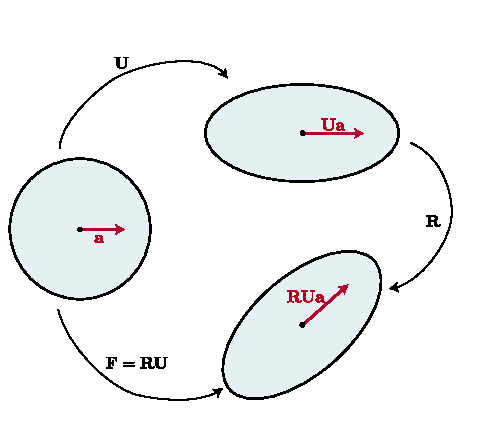
\includegraphics[scale=1.2]{figure/cinematica/polar}
	\caption{Effect of the polar decomposition. The action of $\Fb$ on the vector $\ab$ can be decomposed as the action of a pure deformation $\Ub$ followed by a rotation $\Rb$.}
	\label{fig:polar}
\end{figure}
%
In this sense, $\Fb$ \textit{is not} a good \textit{measure of strain}. The tensors $\Cb$ and $\Ub$ are instead suitable for describing the shape changes of bodies associated with metric variations. However, they do not vanish in the case of rigid deformations. In fact, if $\Fb = \Rb$, then $\Cb = \Ub = \Ib$. Since it makes sense to define the strain measure as a defect of rigidity, we introduce the \textit{Green--Saint-Venant tensor}
\begin{definition}
	\begin{equation}
		\Eb_{\rm G} \coloneqq \frac{1}{2}(\Cb - \Ib),
	\end{equation}
\end{definition}
which corresponds to a rigid deformation with the null tensor. The factor $1/2$ does not have a physical meaning, but it will be convenient later.


Analogously, we can introduce the  \textit{ left polar decomposition}
\begin{definition}
\begin{equation}
	\Fb=\Vb\Rb
\end{equation}
\end{definition}
where 
\begin{equation}
 \Vb=\sqrt{\Fb\Fb^\top}.
\end{equation}
is \textit{left stretch tensor}. The tensor
\begin{equation}
\Bb=\Vb^2= \Fb\Fb^\top
\end{equation}
is the  \textit{left Cauchy--Green} (deformation) tensor.




\section{Deformation in curvilinear coordinates}
	Let us consider a set of curvilinear coordinates $\zeta^i$ $(i=1,2,3)$ for a point $\xb\in\Vr$:
	\begin{equation}
		(\zeta^1,\zeta^2,\zeta^3)\mapsto \xb=\widehat{\xb}(\zeta^1,\zeta^2,\zeta^3), \qquad \xb\mapsto\zeta^i=\widehat{\zeta}^i (\xb)\;(i=1,2,3),
	\end{equation}
	with
	\begin{equation}
		\widehat{\xb}\big(\widehat\zeta^1(\xb),\widehat\zeta^2(\xb),\widehat\zeta^3(\xb)\big)=\xb.
	\end{equation}
	Let $\yb$ be the image of $\xb$ under the deformation $\fb$. To the point $\yb$ we associate the same set of curvilinear coordinates $\zeta^i$ $(i=1,2,3)$:
	\begin{equation}
		(\zeta^1,\zeta^2,\zeta^3)\mapsto \yb=\widehat{\yb}(\zeta^1,\zeta^2,\zeta^3), \qquad y\mapsto\zeta^i=\widehat{\zeta}^i(\yb) \;(i=1,2,3).
	\end{equation}
	For this reason, $\zeta^i$ are called \textit{convected curvilinear coordinates}.
	
We call  \textit{covariant} a basis made of tangent vectors to the coordinate lines:
\begin{equation}
\gb_i=\partial_{\zeta^i}\xb,
\end{equation}
while \textit{contravariant} the basis made of the gradients of the coordinate functions:
\begin{equation}
\gb^i=\partial_\xb\zeta^i.
\end{equation}
\begin{figure}
	\centering
	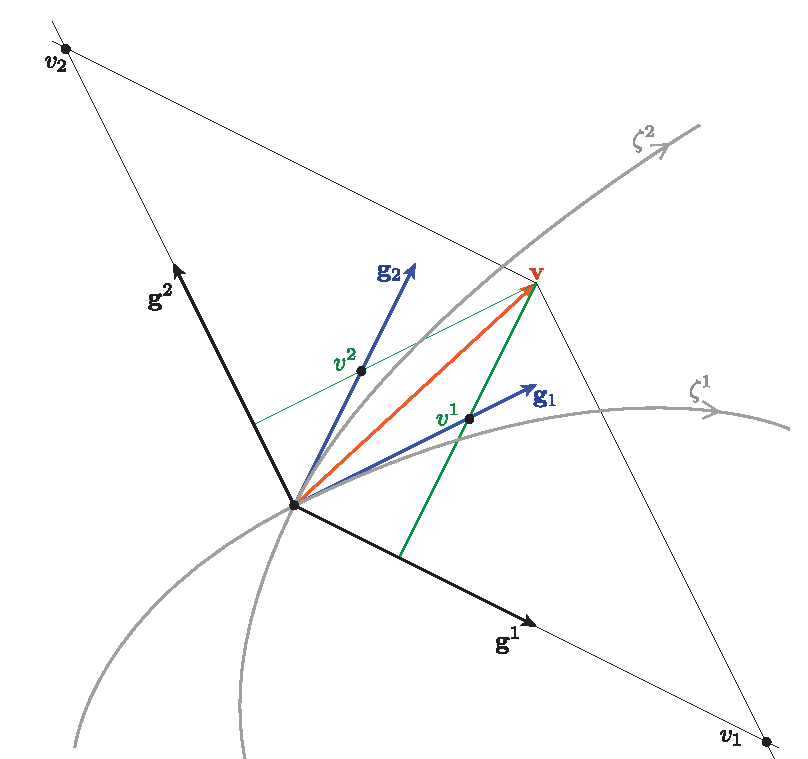
\includegraphics[scale=0.7]{figure/cinematica/covariante}
\caption{A set of non-orthogonal coordinates. The vectors of the covariant basis $\gb_1$ are tangent to the coordinate lines, while the vectors of the contravariant basis $\gb_{i}$ are such that $\gb_1\cdot \gb^2=0$ and $\gb_2\cdot\gb^1=0$. }
	\label{fig:covariante}
\end{figure}



	
	The deformation gradient can be determined as
\begin{definition}
		\begin{equation}\label{Fdy}
		\Fb=\partial_\xb \yb=(\partial_{\zeta^i} \yb)\,(\partial_\xb\zeta^i)=\hb_i\otimes\gb^i, \quad \hb_i:=\partial_{\zeta^i} \yb, \;\gb^i:=\partial_\xb\zeta^i,
	\end{equation}
\end{definition}
	where the vectors $\gb^i\in\Vr$ compose the \textit{contravariant base} in the reference placement and the vectors $\hb_i\in\Vcu$ compose the covariant base in the current placement. It is worth noticing that 
	\begin{equation}
	\partial_{\zeta^j}\zeta^i=\delta^{i}_j,
	\end{equation}
where $\delta^{i}_j$ is the Dirac delta. Therefore
	\begin{equation}
		(\partial_\xb\zeta^i)\cdot(\partial_{\zeta^j}\xb)=\delta^i_j \qquad \gb^i\cdot\gb_j={\delta}^i_j,
	\end{equation}
	where $\gb_j$ define the covariant base in the reference placement. Since
	\begin{equation}
		\Fb\gb_i=\hb_i,
	\end{equation}
	it is evident that $\Fb$ transforms the covariant base in $\Vr$ into the covariant base in $\Vcu$.
	
	In this way it is also evident that $\Fb^\top$, which has the dyadic representation
	\begin{equation}
		\Fb^\top=\gb^i\otimes\hb_i
	\end{equation}
	maps $\Vcu$ into $\Vr$. Similarly, we have that
	\begin{equation}
		\Fb^{-1}=\gb_i\otimes\hb^i,
	\end{equation}
	maps   $\Vcu$ into $\Vr$.

We can also see that $\Fb\Fb^{-1}$ and $\Fb^{-1}\Fb$ are not the same object:
\begin{equation}
\Fb\Fb^{-1}=(\hb_i\otimes\gb^i)(\gb_i\otimes\hb^i)=\hb_i\otimes\hb^i=\Ib_{\rm cur},
\end{equation}
\textit{i.e.}, the \textit{metric tensor} in the current configuration, while 
\begin{equation}
\Fb^{-1}\Fb=(\gb_i\otimes\hb^i)(\hb_i\otimes\gb^i)=\gb_i\otimes \gb^i=\Ib_{\rm ref},
\end{equation}
\textit{i.e.}, the \textit{metric tensor} in the referential configuration.

Finally, since
	\begin{equation}
		\Cb=\Fb^\top\Fb=(\gb^i\otimes\hb_i)(\hb_j\otimes\gb^j)=(\hb_i\cdot\hb_j)\gb^i\otimes\gb^j,
	\end{equation}
	\begin{equation}
		\Bb=\Fb\Fb^\top= (\hb_i\otimes\gb^i)(\gb^j\otimes\hb_j)=(\gb^i\cdot\gb^j)\hb_i\otimes\hb_j.
	\end{equation}
	we conclude that $\Cb$ is a linear transformation of $\Vr$ into itself, while $\Bb$ is  a linear transformation of $\Vcu$ into itself.



\begin{exercise}
	Given the following deformation gradient:
	\begin{equation}
		\Fb = -\frac{1}{2}(\alpha + \beta)\eb_1 \otimes \eb_1 + \frac{1}{2}(\alpha - \beta)\eb_2 \otimes \eb_2 - \frac12 (\alpha + \beta)(\eb_1 \otimes \eb_2 - \eb_2 \otimes \eb_1) + \gamma \,\eb_3 \otimes \eb_3,
	\end{equation}
	with $\alpha, \beta$, and $\gamma$ positive constants. Determine the polar decomposition of $\Fb$.
	\begin{svolgimento}
		The matrix representation of $\Fb$ is 
		\begin{equation}
			[\Fb]= \left[
			\begin{array}{ccc}
				-\dfrac{\alpha + \beta}{2} & -\dfrac{1}{2} (\alpha + \beta ) & 0 \\ [.2cm]
				\dfrac{\alpha + \beta}{2} & \dfrac{\alpha - \beta}{2} & 0 \\[.2cm]
				0 & 0 & \gamma  \\
			\end{array}
			\right]
		\end{equation}
		A simple calculation shows that the representative matrix of the right Cauchy-Green tensor $\Cb = \Fb^\top \Fb$ is
		\begin{equation}
			[\Cb]=\left[
			\begin{array}{ccc}
				\dfrac{1}{2} \left(\alpha^2 + \beta^2\right) & \dfrac{1}{2} (\alpha - \beta ) (\alpha + \beta ) & 0 \\[.2cm]
				\dfrac{1}{2} (\alpha - \beta ) (\alpha + \beta ) & \dfrac{1}{2} \left(\alpha^2 + \beta^2\right) & 0 \\[.2cm]
				0 & 0 & \gamma^2 \\
			\end{array}
			\right]
		\end{equation}
		We now determine the eigenvalues of $\Cb$, solving the characteristic polynomial
		\begin{equation}
			\det(\Cb - \lambda \Ib) = \left(\gamma^2 - \lambda \right) \left(\alpha^2 \beta^2 - \alpha^2 \lambda - \beta^2 \lambda + \lambda^2\right),
		\end{equation}
		whose solutions are
		\begin{equation}
			\lambda_1 = \alpha^2, \quad \lambda_2 = \beta^2, \quad \lambda_3 = \gamma^2.
		\end{equation}
		The corresponding eigenvectors are
		\begin{equation}
			\cb_1 = \frac{1}{\sqrt{2}}(\eb_1 + \eb_2), \quad \cb_2 = \frac{1}{\sqrt{2}}(-\eb_1 + \eb_2), \quad \cb_3 = \eb_3.
		\end{equation}
		The spectral representation of $\Cb$ is thus
		\begin{equation}
			\Cb = \alpha^2 \, \cb_1 \otimes \cb_1 + \beta^2 \, \cb_2 \otimes \cb_2 + \gamma^2 \eb_3 \otimes \eb_3,
		\end{equation}
		and therefore
		\begin{equation}
			\Ub = \alpha \, \cb_1 \otimes \cb_1 + \beta \, \cb_2 \otimes \cb_2 + \gamma \, \eb_3 \otimes \eb_3.
		\end{equation}
		The inverse of $\Ub$ is immediately found:
		\begin{equation}
			\Ub^{-1} = \frac{1}{\alpha} \, \cb_1 \otimes \cb_1 + \frac{1}{\beta} \, \cb_2 \otimes \cb_2 + \frac{1}{\gamma} \, \eb_3 \otimes \eb_3,
		\end{equation}
		or, recalling the expression for the eigenvectors,
		\begin{equation}
			\Ub^{-1} = \left[
			\begin{array}{ccc}
				\dfrac{\alpha + \beta}{2 \alpha \beta} & \dfrac{1}{2} \left(\dfrac{1}{\alpha} - \dfrac{1}{\beta}\right) & 0 \\[.2cm]
				\dfrac{1}{2} \left(\dfrac{1}{\alpha} - \dfrac{1}{\beta}\right) & \dfrac{\alpha + \beta}{2 \alpha \beta} & 0 \\[.2cm]
				0 & 0 & \dfrac{1}{\gamma} \\
			\end{array}
			\right].
		\end{equation}
		The rotation tensor has the following matrix representation:
		\begin{equation}
			[\Rb] = [\Fb][\Ub^{-1}] = \left[
			\begin{array}{ccc}
				0 & -1 & 0 \\
				1 & 0 & 0 \\
				0 & 0 & 1 \\
			\end{array}
			\right].
		\end{equation}
		The polar decomposition is therefore
		\begin{equation}
			\Fb = \Rb \Ub.
		\end{equation}
	\end{svolgimento}
\end{exercise}


\begin{exercise}
	Given the displacement field
	%Libro Capecchi
	\begin{equation}
		\ub(\xb) = \frac{3}{L}x_1^2\eb_1 + \frac{2}{L^2}x_2x_3^2\eb_2 + \frac{1}{L^2}x_1x_3^2\eb_3.
	\end{equation}
	\begin{enumerate}
		\item Determine the position of the point $P$ that before the deformation occupied the position $\xb = L\eb_1 + 2L\eb_3$.
		\item Determine the deformation $\fb(\xb)$, the deformation gradient $\Fb(\xb)$, the displacement gradient $\Hb(\xb)$, the right Cauchy-Green tensor $\Cb(\xb)$, and the Green-Saint-Venant deformation tensor $\Eb_{\rm G}(\xb)$ at point $P$.
		\item Determine if the deformation is homogeneous.
		\item Calculate the relative length change $dl/dl_0$ in the direction $\eb_1$ and the relative volume change $dv/dv_0$ at point $P$.
	\end{enumerate}
	\begin{svolgimento}
		\begin{enumerate}
			\item The deformation is easily found as
			\begin{equation}
				\fb(\xb) = \ub(\xb) + \xb = \left(x_1 + \frac{3}{L}x_1^2\right)\eb_1 + \left(x_2 + \frac{2}{L^2}x_2x_3^2\right)\eb_2 + \left(x_3 + \frac{1}{L^2}x_1x_3^2\right)\eb_3.
			\end{equation}
			Thus, the position of point $P$ after deformation is
			\begin{equation}
				\yb(P) = \fb(\xb(P)) = 2L(2\eb_1 + 3\eb_3).
			\end{equation}
			\item
			Using the definition, we have
			\begin{equation}
				\begin{aligned}
					\Fb(\xb) &= \fb{,_i} \otimes \eb_i = \left(1 + \frac{6x_1}{L}\right)\eb_1 \otimes \eb_1 + \frac{x_3^2}{L^2}\eb_3 \otimes \eb_1 + \left(1 + \frac{2x_3^2}{L^2}\right)\eb_2 \otimes \eb_2 \\
					&+ \frac{4x_2x_3}{L^2} \eb_2 \otimes \eb_3 + \left(1 + \frac{2x_1x_3}{L^2}\right)\eb_3 \otimes \eb_3.
				\end{aligned}
			\end{equation}
			Alternatively, considering the components, remembering that $F_{ij} = f_{i,j}$,\footnote{Recall that $f_{i,j}$ means $\frac{\partial f_i}{\partial x_j}$.} the representative matrix of $\Fb$ is
			\begin{equation}
				[\Fb(\xb)] = \left[\begin{matrix}
					1 + \frac{6x_1}{L} & 0 & 0 \\
					0 & 1 + \frac{2x_3^2}{L^2} & \frac{4x_2x_3}{L^2} \\
					\frac{x_3^2}{L^2} & 0 & 1 + \frac{2x_1x_3}{L^2}
				\end{matrix}\right].
			\end{equation}
			Evaluating $\Fb$ at point $P$, we get
			\begin{equation}
				\Fb(\xb(P)) = 7\eb_1 \otimes \eb_1 + 9\eb_2 \otimes \eb_2 + 4\eb_3 \otimes \eb_1 + 5\eb_3 \otimes \eb_3.
			\end{equation}
			Similarly, for $\Hb(\xb)$, once $\Fb(\xb)$ is calculated, we remember that $\Hb = \Fb - \Ib$:
			\begin{equation}
				\Hb(\xb) = \left(\frac{6x_1}{L}\right)\eb_1 \otimes \eb_1 + \frac{x_3^2}{L^2}\eb_3 \otimes \eb_1 + \left(\frac{2x_3^2}{L^2}\right)\eb_2 \otimes \eb_2 + \frac{4x_2x_3}{L^2}\eb_2 \otimes \eb_3 + \left(\frac{2x_1x_3}{L^2}\right)\eb_3 \otimes \eb_3.
			\end{equation}
			%
			Finally, the right Cauchy-Green tensor is determined as
			\begin{equation}
				\Cb(\xb(P)) = 65\eb_1 \otimes \eb_1 + 20(\eb_1 \otimes \eb_3 + \eb_3 \otimes \eb_2) + 81\eb_2 \otimes \eb_2 + 25\eb_3 \otimes \eb_3,
			\end{equation}
			and the Green-Saint-Venant tensor is
			\begin{equation}
				\Eb_{\rm G}(\xb(P)) = \frac{1}{2}(\Cb(\xb(P)) - \Ib) = \Big( 32\eb_1 \otimes \eb_1 + 10(\eb_1 \otimes \eb_3 + \eb_3 \otimes \eb_2) + 40\eb_2 \otimes \eb_2 + 12\eb_3 \otimes \eb_3 \Big).
			\end{equation}
			\item Since $\Fb(\xb)$ is not constant, the deformation is not homogeneous.
			\item The relative length change at point $P$ in the direction $\eb_1$ is
			\begin{equation}
				\frac{d\ell}{d\ell_0} = |\Fb(\xb(P)) \eb_1| = \sqrt{65},
			\end{equation}
			while the relative volume change is
			\begin{equation}
				\frac{dv}{dv_0} = \det(\Fb(\xb(P))) = 315.
			\end{equation}
		\end{enumerate}
	\end{svolgimento}
\end{exercise}

\begin{exercise}
	Let $\rb : [0,2\pi] \mapsto \Omega$ be the cylindrical helix parametrized by
	\begin{equation}
		\rb(\theta) = \cos\theta \eb_1 + \sin\theta \eb_2 + \theta \eb_3
	\end{equation}
	and let $\fb$ be the deformation
	\begin{equation}
		\fb(\xb) = x_2 \eb_1 + x_1 \eb_2 + 2x_3 \eb_3.
	\end{equation}
	\begin{enumerate}
		\item Determine the deformation gradient $\Fb(\xb)$ and the right Cauchy-Green tensor $\Cb(\xb)$.
		\item Calculate the lengths $\ell_0$ of the undeformed helix and $\ell$ of the deformed helix.
	\end{enumerate}
	
	\begin{svolgimento}
		\begin{enumerate}
			\item Using the definition, we immediately calculate
			\begin{equation}
				\Fb(\xb) = \fb{,_i}(\xb) \otimes \eb_i = \eb_2 \otimes \eb_1 + \eb_1 \otimes \eb_2 + 2\eb_3 \otimes \eb_3.
			\end{equation}  
			On the other hand, using the component representation and recalling that $F_{ij} = f_{i,j}$, we find
			\begin{equation}
				[\Fb] = \left[
				\begin{matrix}
					0 & 1 & 0 \\
					1 & 0 & 0 \\
					0 & 0 & 2
				\end{matrix}
				\right].
			\end{equation}
			Finding the Cauchy-Green tensor is straightforward:
			\begin{equation}
				\Cb = \Fb^\top \Fb = \eb_1 \otimes \eb_1 + \eb_2 \otimes \eb_2 + 4 \eb_3 \otimes \eb_3,
			\end{equation}
			or
			\begin{equation}
				[\Cb] = [\Fb^\top \Fb] = \left[
				\begin{matrix}
					1 & 0 & 0 \\
					0 & 1 & 0 \\
					0 & 0 & 4
				\end{matrix}
				\right].
			\end{equation}
			
			\item The generic point of the helix is given by $\rb(\theta)$, varying with $\theta \in [0, 2\pi]$. To find the initial length of the helix, we use the formula for calculating the length of a curve:
			\begin{equation}
				\ell_0 = \int_0^{2\pi} |\rb'(\theta)| d\theta = 2\sqrt{2} \pi.
			\end{equation}
			Due to the deformation, the generic point of the helix is mapped to
			\begin{equation}
				\yb = \fb(\rb(\theta)) = \sin\theta \eb_1 + \cos\theta \eb_2 + 2\theta \eb_3.
			\end{equation}
			The length of the deformed helix is then
			\begin{equation}
				\ell = \int_0^{2\pi} |\yb'(\theta)| d\theta = 2\sqrt{5} \pi.
			\end{equation}
		\end{enumerate}
	\end{svolgimento}
	
\end{exercise}

\begin{exercise}
Let us consider 
		the curvilinear cylindrical coordinates $(\zeta^1=\rho,\zeta^2=\varphi,\zeta^3=x_3)$; the position vector of point $x$ is then
		$$
		\xb=x-o=\rho\eb(\varphi)+x_3\eb_3, \quad \eb(\varphi):=\cos\varphi\eb_1+\sin\varphi \eb_2.
		$$
Determine the covariant and contravariant basis.

\begin{svolgimento}
			The covariant vector basis is:
		\begin{equation}
			\gb_1=\partial_{\zeta^1}\xb=\eb(\varphi), \quad \gb_2=\partial_{\zeta^2}\xb=\rho\eb'(\varphi), \quad \gb_3=\partial_{\zeta^3}\xb=\eb_3.
		\end{equation}
		To determine the contravariant vector basis, we notice that
		$$
		x_1=\xb\cdot\eb_1=\rho\cos\varphi, \quad x_2=\xb\cdot\eb_2=\rho\sin\varphi;
		$$
		since $\rho^2=x_1^2+x_2^2$, and $\tan\varphi=\frac{x_2}{x_1}$, we get
		$$
		\gb^1=\partial_\xb\zeta^1=\nabla\rho=\frac{x_1}{\rho}\eb_1+\frac{x_2}{\rho}\eb_2=\eb(\varphi), \quad 
		\gb^2=\partial_\xb\zeta^2=\nabla\varphi=\frac{1}{\rho}\eb'(\varphi).
		$$
\end{svolgimento}
	
\end{exercise}

\section{Motion velocity, velocity gradient, stretching, and spin}
On introducing the time variable $t\in\Ro^+$, we use the following notation:\\
\noindent for a \textit{motion},
\begin{equation}
	(\xb,t)\mapsto \yb=\fb(\xb,t)=:\fb_t(\xb);
\end{equation} 
for the deformation gradient and the \textit{motion velocity} $\vb$
\begin{equation}
	\Fb=\partial_\xb \yb, \qquad \vb=\partial_t \yb.
\end{equation}

Let us consider a \textit{referential} field $\varphi=\phi(\xb,t)$; we will use the notation
\begin{equation}
	\nabla\varphi=\partial_\xb\varphi, \qquad \dot{\varphi}=\partial_t\varphi.
\end{equation}
Some care is needed if the current counterpart of $\varphi$ is considered:
\begin{equation}
	\varphi=\widehat{\varphi}(\yb,t):=\phi\big( \fb_t^{-1}(\yb),t  \big).
\end{equation}
In this case we have
\begin{equation}
	\dot{\varphi}=(\partial_\yb\phi)\partial_t \yb+\partial_t\varphi=(\partial_\yb\varphi)\vb+\partial_t\varphi.
\end{equation}
In order to distinguish the spatial derivative with respect to current point $\yb$, we introduce the following notation
\begin{equation}
	\grad\varphi=\partial_\yb\varphi.
\end{equation}
Then, we have
\begin{equation}
	\dot\varphi=(\grad\varphi)\,\vb+\partial_t\varphi.
\end{equation}
For any field $\varphi$ that is given both a referential and current description, the relation
\begin{definition}
\begin{equation}
	\nabla\varphi=(\grad \varphi)\Fb
\end{equation}
\end{definition}
holds true, as proved by the following sequence of equalities:
\begin{equation}
	\nabla\varphi=\partial_\xb\varphi=(\partial_\yb\varphi)(\partial_\xb \yb)=(\grad \varphi)\Fb.
\end{equation}


We introduce the \textit{velocity gradient} $\Lb$:
\begin{equation}
	\Lb(\yb,t):=\partial_\yb\vb=\grad\vb.
\end{equation}
Now, we have that
\begin{equation}
	\dot{\Fb}=\partial_t(\partial_\xb \yb)=\partial_\xb(\partial_t \yb)=\partial_\xb\vb=(\partial_\yb\vb)(\partial_\xb \yb)=\Lb\Fb,
\end{equation}
and then
\begin{definition}
\begin{equation}
	\Lb=\dot\Fb\Fb^{-1}.
\end{equation}
\end{definition}

%The gradient velocity $\Lb$ tells how velocity varies from point to point in the current configuration: $\dot\Fb$ tells  how the deformation is changing over time at a fixed material point, but we want to know the current rate of change of the velocity field; to do that, we must move from the referential description to the current description, through $\Fb^{-1}$.

It accounts for both stretching and rotation of material elements.


The symmetric and skew-symmetric parts of $\Lb$
\begin{equation}
	\Db=\frac 12 (\Lb+\Lb^\top), \quad \Wb=\frac 12 (\Lb-\Lb^\top)
\end{equation}
are called \textit{stretching tensor} and \textit{spin tensor}; the former is a measure of the \textit{strain rate}, while the latter is a measure of the \textit{motion vorticity}.


%\begin{exercise}
%	A deformation of the form
%	\begin{equation}
%		\begin{aligned}
%			& y_1=x_1+\gamma x_2\\
%			& y_2=x_2,\\
%			& y_3=x_3
%			\end{aligned}
%		\end{equation}
%	is called \emph{pure shear}. For this deformation compute:
%	\begin{enumerate}
%			\item the matrices of $\Fb,\Cb$ and $\Bb$;
%%			\item the list of principal invariants of $\Cb$;\footnote{We recall that, for a second order tensor $\Ab$, the principal invariants are:
%%				$$
%%				I_1=\tr{\Ab}, \quad I_2=\frac{1}{2}\big((\tr{\Ab})^2-\tr{\Ab^2}  \big), \quad I_3=\det\Ab.
%%				$$
%%			They are the coefficients of the  characteristic polynomial $\det(\Ab-\lambda\Ib)$, whose solutions are the eingevalues of $\Ab$.
%%					\item the principal stretches, i.e., the eigenvalues of $\Ub$ or $\Vb$.
%	\end{enumerate}
%\end{exercise}

\begin{exercise}
	Show that a deformation is  \emph{isochoric} (i.e. volume preserving) if $\det\Cb=1$.
\end{exercise}


%\begin{exercise}
%Show that a deformation is rigid if and only if the list of invariants of $\Cb$ is $(3,3,1)$.
%\end{exercise}



\begin{exercise}
	The deformation of a two-dimensional continuum is given as
	$$
	y_1=4-2x_1-x_2; \quad y_2=2+\frac{2}{3}x_1-\frac{1}{2}x_2.
	$$
	\begin{enumerate}
			\item Calculate the deformation gradient tensor $\Fb$, the right Cauchy-Green strain tensor $\Cb$ and the left Cauchy-Green strain tensor $\Bb$.
			\item Calculate the stretch undergone by a unit material vector $\ab_0=\frac{3}{5}\eb_1+\frac{4}{5}\eb_2$ as a result of the deformation.
			\item Demonstrate whether or not the deformation is isochoric. 
		\end{enumerate}
\end{exercise}

\begin{exercise}
	A deformation of the form
$$
	\begin{aligned}
		& y_1=f_1(x_1,x_2)\\
		& y_2=f_2(x_1,x_2),\\
		& y_3=x_3
		\end{aligned}
$$
	is called \textit{plane strain}. Show that for such a deformation the principal stretch $\lambda_3$ (in $x_3$ direction) is unity. Show further that the deformation is isochoric if and only if the other principal stretches, $\lambda_\alpha$ and $\lambda_\beta$ satisfy
	$$
	\lambda_\alpha=\frac{1}{\lambda_\beta}.
	$$
\end{exercise}
%
%
%\begin{exercise}
%	Let 
%	$$
%	\varepsilon=|\Fb-\Ib|=|\nabla\ub|
%	$$
%	a smallness parameter, so that $\Fb(\varepsilon)=\Ib+\varepsilon\nabla\ub$.
%	\begin{enumerate}
	%		\item compute the linear approximation about $\varepsilon=0$ of the Green--St. Venant tensor $\Eb$ and show that
	%		$$
	%		\Eb\simeq\Gb, \qquad \Gb:=\sym\nabla\ub,
	%		$$
	%	i.e., the  strain measure adopted in linear elasticity;
	%	\item show that
	%$$
	%\delta l(\eb)\simeq\eb\cdot\Gb\eb;
	%$$
	%\item show that
	%$$
	%\delta a(\nb_{\rm ref})\simeq\Gb\cdot(\Ib-\nb_{\rm ref}\otimes\nb_{\rm ref})
	%$$
	%\item show that
	%$$
	%\delta v\simeq\Gb\cdot\Ib=\tr{\Eb}.\footnote{To this end, it is useful to recall a formula known to Euler:
		%	$$
		%	\partial_{\Ab}(\det\Ab)=\Ab^*.
		%	$$}
	%$$
	%
	%	\end{enumerate}
%\end{exercise}
%
\begin{exercise}
	Prove that
	$$
	\dot{\Cb}=2\Fb^\top\Db\Fb.
	$$
\end{exercise}


\chapter{Infinitesimal Theory}\label{inf}

From equation \eqref{dl}, it follows that if the deformation gradient is close to the identity, then the variations in length are small. We can thus introduce a smallness parameter, given by
\begin{equation}
	\varepsilon\coloneqq\sup_{\xb\in\Omega}|\Fb(\xb)-\Ib|,
\end{equation}
which measures the greatest distance between \(\Fb\) and the identity. Given the definition of displacement gradient and equation \eqref{HFI}, the parameter can be rewritten as
\begin{equation}\label{eps}
	\varepsilon=\sup_{\xb\in\Omega}|\Hb(\xb)|.
\end{equation}

We now want to consider a theory, called the \textit{infinitesimal theory}, obtained by neglecting infinitesimals of order higher than the first in \(\varepsilon\).


\section{The Infinitesimal Strain Tensor}

First, let's see what the deformation measures are in the infinitesimal theory. We observe that we can write the deformation gradient as
\begin{equation}
	\Fb(\xb)=\Ib +\varepsilon(\xb) \widetilde{\Hb}(\xb), \qquad \varepsilon(\xb)\coloneqq |\Hb(\xb)|, \quad \widetilde{\Hb}(\xb)\coloneqq \frac{\Hb(\xb)}{|\Hb(\xb)|}.
\end{equation}
Given equation \eqref{eps}, certainly
\begin{equation}
	\varepsilon(\xb)\leq \varepsilon \qquad \forall \xb\in \Omega
\end{equation}
and thus we are allowed to neglect terms of order \(\varepsilon^2(\xb)\). Neglecting these terms, the right Cauchy-Green tensor then becomes
\begin{equation}\label{Cap}
	\begin{aligned}
		\Cb(\xb)=	\mathbf{F}^\top(\mathbf{x})\mathbf{F}(\mathbf{x})& =\mathbf{I+H^\top(x)+H(x)}+\frac12\Hb^\top(\xb)\Hb(\xb) \\
		&=\mathbf{I}+\varepsilon(\mathbf{x})\widetilde{\mathbf{H}}^\top(\mathbf{x})+\varepsilon(\mathbf{x})\widetilde{\mathbf{H}}(\mathbf{x})+\frac12\varepsilon^2(\mathbf{x})\widetilde{\mathbf{H}}^\top(\mathbf{x})\widetilde{\mathbf{H}}(\mathbf{x}) \\
		&=\mathbf{I}+\varepsilon(\mathbf{x})\widetilde{\mathbf{H}}^\top(\mathbf{x})+\varepsilon(\mathbf{x})\widetilde{\mathbf{H}}(\mathbf{x}) \\
		&=\mathbf{I+H^\top(x)+H(x)}.
	\end{aligned}
\end{equation}
In the following, we will avoid introducing the parameter \(\varepsilon\) and neglect terms that are superlinear in \(\Hb\).

The Green-Saint-Venant deformation measure thus becomes
\begin{equation}
	\Eb_{\rm G}(\xb)=\frac{1}{2}(\Cb(\xb)-\Ib)=\frac{1}{2}\left(\mathbf{H(x)+H^\top(x)}\right).
\end{equation}

The tensor
\begin{definition}
	\begin{equation}\label{simgrad}
		\Eb(\xb)\coloneqq\sym \Hb(\xb)
	\end{equation}
\end{definition}
is called the \textit{infinitesimal strain tensor}, which will be used to completely characterize the metric variations in infinitesimal theory.

\section{The Infinitesimal Rotation Tensor}

Like any second-order tensor, the displacement gradient can be decomposed into its symmetric and skew-symmetric parts:
\begin{equation}
	\Hb=\sym \Hb+\skw \Hb.
\end{equation}
We have already defined the infinitesimal deformation tensor \(\Eb=\sym \Hb\); now we show that the skew-symmetric part
\begin{definition}
	\begin{equation}
		\Wb\coloneqq\skw \Hb
	\end{equation}
\end{definition}
represents an infinitesimal rigid rotation. To show this, we approximate the relation
\begin{equation}
	\Rb=\Fb\Ub^{-1}
\end{equation}
to see the form of an infinitesimal rotation. Neglecting superlinear terms in \(\Hb\), from \eqref{Cap} we have
\begin{equation}
	\Ub^2=\Cb=\Ib+2\Eb.
\end{equation}
On the other hand, the following chain of equalities holds:
\begin{equation}
	(\Ib+\Eb)^2=(\Ib+\Eb)(\Ib+\Eb)=\Ib+2\Eb=\Ub^2,
\end{equation}
from which we can deduce that
\begin{equation}
	\Ub=\Ib+\Eb.
\end{equation}
Now that we have the approximation for \(\Ub\), we need to find the one for \(\Ub^{-1}\). Since
\begin{equation}
	(\Ib+\Eb)(\Ib-\Eb)=\Ib,
\end{equation}
we can conclude that
\begin{equation}
	\Ub^{-1}=\Ib-\Eb.
\end{equation}
We are now ready to determine the form that a rotation \(\Rb\) takes when superlinear terms in \(\Hb\) (i.e., small deformations) are neglected:
\begin{equation}
	\Rb=\Fb\Ub^{-1}=(\Ib+\Hb)(\Ib-\Eb)=\Ib-\Eb+\Hb=\Ib+\Wb.
\end{equation}
Thus, we conclude that the rotation of a point \(\xb\) around \(\xb_0\) has the following representation in infinitesimal theory:
\begin{equation}
	\Rb(\xb-\xb_0)=(\xb-\xb_0)+\Wb(\xb-\xb_0).
\end{equation}
Since, in a rigid displacement \(\nabla \ub=\Fb-\Ib=\Rb-\Ib=\Wb\), we obtain the following representation of the \textit{infinitesimal rigid displacement} field:
\begin{definition}
	\begin{equation}\label{urig}
		\ub_{\rm rig}(\xb)=\ub(\xb_0)+\Wb (\xb-\xb_0).
	\end{equation}
\end{definition}
Since an skew-symmetric tensor \(\Wb\) can be associated with a vector \(\wb\), according to the following correspondence
\begin{equation}
	\Wb \ab=\wb \times \ab \quad \forall \ab\in \Vc,
\end{equation}
\eqref{urig} can be equivalently rewritten as
\begin{definition}
	\begin{equation}\label{urig}
		\ub_{\rm rig}(\xb)=\ub(\xb_0)+\wb \times(\xb-\xb_0).
	\end{equation}
\end{definition}
The vector \(\wb\) is called the \textit{axial} vector of \(\Wb\). Its unit vector \(\wb/|\wb|\) represents the axis of rotation, while its magnitude gives the (infinitesimal) angle of rotation.

\begin{remark}\label{skvec}
	Let us choose a Cartesian basis \(\{\eb_i\}\) and represent the tensor \(\Wb\in\Skw\) in matrix form:
	\begin{equation}
		[\Wb]=\left[\begin{array}{ccc}0&-\gamma&\beta\\\gamma&0&-\alpha\\-\beta&\alpha&0\end{array}\right].
	\end{equation}
	A simple calculation shows that the axial vector of \(\Wb\) is then
	\begin{equation}
		\wb=\alpha\eb_1+\beta\eb_2+\gamma\eb_3.
	\end{equation}
\end{remark}

Both \(\Rb\) and \(\Wb\) are constant tensors, having considered a homogeneous deformation. However, the general deformation \(\fb(\xb)\) of a point \(\xb\) can be expanded in a series around another point \(\xb_0\):
\begin{equation}
	\fb(\xb)=\fb(\xb_0)+\Fb(\xb_0)(\xb-\xb_0)+o(|\xb-\xb_0|).
\end{equation}
This means that in the neighborhood of a point \(\xb\), to an error of the order \(o(|\xb-\xb_0|)\), any deformation behaves as if it were homogeneous. This justifies the following terminology: let
\begin{equation}
	\Fb(\xb)=\Rb(\xb)\Ub(\xb)
\end{equation}
be the \textit{local} polar decomposition for \(\Fb(\xb)\); then \(\Rb(\xb)\) is the \textit{local} rotation tensor and \(\Ub(\xb)\) the \textit{local} Cauchy-Green tensor. \(\Rb(\xb)\) is a measure of the local rigid rotation of points close to \(\xb\), while \(\Ub(\xb)\) is a measure of the deformation around \(\xb\).

Similarly, in infinitesimal theory, we can say that
\begin{equation}
	\Hb(\xb)=\Eb(\xb)+\Wb(\xb)
\end{equation}
is the \textit{local} decomposition of the displacement gradient; the tensor \(\Eb(\xb)\) is the \textit{local} infinitesimal deformation tensor, and \(\Wb(\xb)\) is the \textit{local} infinitesimal rotation tensor. \(\Eb(\xb)\) is a measure of the infinitesimal deformation around \(\xb\), and \(\Wb(\xb)\) is a measure of the local rigid infinitesimal rotation of points close to \(\xb\).



\section{Geometric Changes}

\subsection{Change in Length}
Recalling \eqref{dl}, the ratio between the deformed and undeformed length of an infinitesimal segment in the direction $\tb$, neglecting the superlinear terms in $\Hb$, can be calculated as
\begin{equation}
	\frac{d\ell}{d\ell_0}=|\Fb\tb|=\sqrt{\Cb\tb\cdot\tb}=\sqrt{(\Ib+2\Eb)\tb\cdot\tb}=(\Ib+\Eb)\tb\cdot\tb=1+\Eb\tb\cdot\tb.
\end{equation}
Therefore, in infinitesimal theory, the specific variation in length in the direction $\tb$ is
\begin{definition}
	\begin{equation}\label{Ett}
		\frac{d\ell-d\ell_0}{d\ell_0}=\frac{d\ell}{d\ell_0}-1=\Eb\tb\cdot\tb.
	\end{equation}
\end{definition}

\subsection{Change in Volume}
Without loss of generality, consider a volume element generated by the base vectors, so that $dv_0=\eb_1\times\eb_2\cdot\eb_3=1$. The deformed volume will then be
\begin{equation}
	\begin{aligned}
		dv&=\Fb\eb_1\times\Fb\eb_2\cdot\Fb\eb_3=\det\mathbf{F}=\det(\Ib+\Hb)=(\Ib+\Hb)\eb_1\times(\Ib+\Hb)\eb_2\cdot(\Ib+\Hb)\eb_3\\
		&=\mathbf{e}_{1}\times\mathbf{e}_{2}\cdot\mathbf{e}_{3}+\mathbf{H}\mathbf{e}_{1}\times\mathbf{e}_{2}\cdot\mathbf{e}_{3}+\mathbf{e}_{1}\times\mathbf{H}\mathbf{e}_{2}\cdot\mathbf{e}_{3}+\mathbf{e}_{1}\times\mathbf{e}_{2}\cdot\mathbf{H}\mathbf{e}_{3}\\
		&=1+\mathbf{e}_{2}\times\mathbf{e}_{3}\cdot\mathbf{H}\mathbf{e}_{1}+\mathbf{e}_{3}\times\mathbf{e}_{1}\cdot\mathbf{H}\mathbf{e}_{2}+\mathbf{e}_{1}\times\mathbf{e}_{2}\cdot\mathbf{H}\mathbf{e}_{3}\\
		&=1+\mathbf{H}\mathbf{e}_{1}\cdot\mathbf{e}_{1}+\mathbf{H}\mathbf{e}_{2}\cdot\mathbf{e}_{2}+\mathbf{H}\mathbf{e}_{3}\cdot\mathbf{e}_{3}=1+\operatorname{tr}\mathbf{H}=1+\operatorname{tr}\mathbf{E},
	\end{aligned}
\end{equation}
since $\operatorname{tr}\Wb=0$. It follows that, in infinitesimal theory, the volume variation is
\begin{equation}
	\frac{dv}{dv_0}=1+\operatorname{tr}\Eb,
\end{equation}
that is,
\begin{definition}
	\begin{equation}\label{trE}
		\frac{dv-dv_0}{dv_0}=\operatorname{tr}\mathbf{E}.
	\end{equation}
\end{definition}

\subsection{Change in Area}
Without loss of generality, suppose we consider an area generated by the vectors $\eb_1$ and $\eb_2$, whose reference normal is $\nb_{\rm ref}=\eb_1\times\eb_2=\eb_3$. The initial infinitesimal area is $da_0=|\nb_{\rm ref}|=1$. Neglecting superlinear terms in $\Hb$, the deformed area is
\begin{equation}
	\begin{aligned}
		da&=|\Fb\eb_1\times\Fb\eb_2|=|(\Ib+\Hb)\eb_1\times(\Ib+\Hb)\eb_2|\\
		&=\sqrt{1+2\eb_3\cdot(\eb_1\times\Hb\eb_2+\Hb\eb_1\times\eb_2)}=\sqrt{1+2(\Hb\eb_1\cdot\eb_1+\Hb\eb_2\cdot\eb_2)}\\
		&=1+E_{11}+E_{22}=1+(\Ib-\eb_3\otimes\eb_3)\cdot\Eb.
	\end{aligned}
\end{equation}
Thus, we conclude that, if $\nb_{\rm ref}$ is the reference normal to the surface, then
\begin{definition}
	\begin{equation}\label{da}
		\frac{da-da_0}{da_0}=\frac{da}{da_0}-1=(\Ib-\nb_{\rm ref}\otimes\nb_{\rm ref})\cdot\Eb,
	\end{equation}
\end{definition}
that is, the specific variation in area is equal to the trace of the strain tensor restricted to the plane in which the considered area lies.

\subsection{Change in Angle}
Consider two orthogonal vectors $\eb_{1}$ and $\eb_2$ passing through the same point. The initial angle is $\alpha_0=\pi/2$, while after deformation,
\begin{equation}
	\alpha=\arccos\left(\frac{\mathbf{F^{\top}Fe}_1\cdot\mathbf{e}_2}{|\mathbf{F^{\top}Fe}_1\cdot\mathbf{e}_1|^{1/2}|\mathbf{F^{\top}Fe}_2\cdot\mathbf{e}_2|^{1/2}}\right).
\end{equation}
Since
\begin{equation}
	\mathbf{F^{\top}Fe}_1\cdot\mathbf{e}_2=(\mathbf{I}+2\mathbf{E})\mathbf{e}_1\cdot\mathbf{e}_2=2\mathbf{Ee}_1\cdot\mathbf{e}_2
\end{equation}
and 
\begin{equation}
	\mathbf{|F^{\top}Fe}_1\cdot \eb_1|^{1/2}=\mathbf{|(I+2E)e}_1\cdot \eb_1|^{1/2}=(1+2\Eb\eb_1\cdot \eb_2)^{1/2}=1+\Eb\eb_1\cdot \eb_1
\end{equation}
we get
\begin{equation}
	\begin{aligned}
		\cos\alpha & =\frac{2\mathbf{Ee}_1\cdot\mathbf{e}_2}{(1+\mathbf{Ee}_1\cdot\mathbf{e}_1)(1+\mathbf{Ee}_2\cdot\mathbf{e}_2)}=\frac{2\mathbf{Ee}_1\cdot\mathbf{e}_2}{1+\mathbf{Ee}_1\cdot\eb_1+\mathbf{Ee}_2\cdot\eb_2}  \\
		&=\frac{2\mathbf{Ee}_1\cdot\eb_2}{1+\mathbf{Ee}_1\cdot\eb_1+\mathbf{Ee}_2\cdot\eb_2}\frac{1-\mathbf{Ee}_1\cdot\eb_1-\mathbf{Ee}_2\cdot\eb_2}{1-\mathbf{Ee}_1\cdot\eb_1-\mathbf{Ee}_2\cdot\eb_2} \\
		&=2\mathbf{Ee}_1\cdot\eb_2(1-\mathbf{Ee}_1\cdot\eb_1-\mathbf{Ee}_2\cdot\eb_2) \\
		&=2\mathbf{Ee}_1\cdot\eb_2.
	\end{aligned}
\end{equation}
We now calculate the variation in angle
\begin{equation}
	\delta\alpha=\alpha-\alpha_0=\alpha-\frac{\pi}{2}.
\end{equation}
Since
\begin{equation}
	\sin(\delta\alpha)=\sin(\frac\pi2-\alpha)=\cos\alpha,
\end{equation}
we get
\begin{equation}
	\begin{aligned}\delta\alpha&=\arcsin(\cos\alpha)=\arcsin(2\mathbf{Ee}_1\cdot\mathbf{e}_2)=2\mathbf{Ee}_1\cdot\mathbf{e}_2,\end{aligned}
\end{equation}
which is obtained using the Taylor series expansion of the arcsine: $\arcsin x=x+o(x)$ as $x\to 0$, and therefore
\begin{definition}
	\begin{equation}\label{E12}
		\begin{aligned}\delta\alpha=2\mathbf{Ee}_1\cdot\mathbf{e}_2,\end{aligned}
	\end{equation}
\end{definition}

\section{Components of the Infinitesimal Strain Tensor}
Given a Cartesian basis $\{\eb_i\}$, the infinitesimal strain tensor can be represented in matrix form as follows:
\begin{equation}
	[\Eb]=\begin{bmatrix}E_{11}&E_{12}&E_{13}\\E_{21}&E_{22}&E_{23}\\E_{31}&E_{32}&E_{33}\end{bmatrix}=\begin{bmatrix}E_{11}&E_{12}&E_{13}\\&E_{22}&E_{23}\\\mathrm{sym}&&E_{33}\end{bmatrix}.
\end{equation}

The interpretation of $E_{11}$ is immediate, recalling \eqref{Ett}:
\begin{equation}
	E_{11}=\Eb\eb_1\cdot\eb_1=\frac{d\ell-d\ell_0}{d\ell_0},
\end{equation}
that is, it represents the specific elongation along the direction $\eb_1$. An analogous interpretation can be given for all the diagonal components.

To interpret $E_{12}$, we need to refer to \eqref{E12}: 
\begin{equation}
	E_{12}=\Eb\eb_1\cdot\eb_2=\frac{\delta\alpha}{2},
\end{equation}
that is, it represents half the shear angle between the directions $\eb_1$ and $\eb_2$. A similar interpretation can be given for $E_{13}$ and $E_{23}$.

We also observe that $\operatorname{tr}\Eb=E_{11}+E_{22}+E_{33}$, as per \eqref{trE}, represents the specific variation in an infinitesimal volume generated by the three base vectors. Finally, in light of \eqref{da}, the sum $E_{11}+E_{22}$ represents the specific variation in area in the plane generated by $\eb_1$ and $\eb_2$; a similar interpretation applies to the sum of any pair of elements from the main diagonal.

\section{Elementary Deformations}
In this section, we analyze some significant homogeneous deformations.

\subsubsection{Uniform Extension}
In a uniform extension of $\varepsilon$ in the direction $\nb$ ($|\nb|=1$), the displacement field is given by
\begin{equation}
	\mathbf{u}(\mathbf{x})=\varepsilon\,\mathbf{n}\otimes\mathbf{n}(\mathbf{x}-\mathbf{x}_{0}).
\end{equation}
The generic point $\mathbf{x}$ thus moves in the direction of $\nb$, linearly increasing as $\mathbf{x}$ moves away from the fixed point $\mathbf{x}_0$.

\begin{center}
	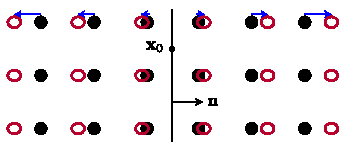
\includegraphics[scale=1.3]{figure/cinematica/estensione}
\end{center}

In this case, 
\begin{equation}
	\nabla\mathbf{u}=\varepsilon\,\mathbf{n}\otimes\mathbf{n}=\mathbf{E}.
\end{equation}
Since
\begin{equation}
	\varepsilon=\mathbf{E}\mathbf{n}\cdot\mathbf{n},
\end{equation}
the constant $\varepsilon$ represents the specific elongation in the direction of $\nb$. 

If $\mathbf{m}$ is a vector orthogonal to $\nb$, since $\mathbf{E}\mathbf{n} \cdot\mathbf{m}=0$, the angle between a fiber directed as $\nb$ and one as $\mathbf{m}$ does not change. Moreover, since $\mathbf{E}\mathbf{m} \cdot\mathbf{m}=0$, there is no variation in length in the direction of $\mathbf{m}$.

\subsubsection{Uniform Dilation}
In a dilation of $\kappa$ around $\mathbf{x}_0$, the displacement field is
\begin{equation}
	\mathbf{u}(\mathbf{x})=\kappa(\mathbf{x}-\mathbf{x}_0).
\end{equation}
All points thus move in the radial direction $\mathbf{x} -\mathbf{x}_0$, by an amount that increases linearly as one moves away from $\mathbf{x}_0$.

\begin{center}
	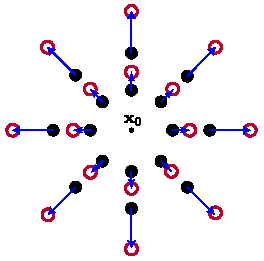
\includegraphics[scale=1.3]{figure/cinematica/dilatazione}
\end{center}

In this case,
\begin{equation}
	\nabla\mathbf{u}=\kappa \mathbf{I}=\mathbf{E}.
\end{equation}
A fiber in any direction $\mathbf{t}$ has a specific elongation
\begin{equation}
	\mathbf{E}\mathbf{t}\cdot\mathbf{t}=\kappa.
\end{equation}
The specific change in volume is
\begin{equation}
	\frac{dv-dv_0}{dv}=\operatorname{tr}\mathbf{E}=3\kappa.
\end{equation}

\subsubsection{Shear}
Consider a point $\mathbf{x}_0$ and two mutually orthogonal unit vectors $\mathbf{n}$ and $\mathbf{m}$. In a shear along $\mathbf{n}$ and $\mathbf{m}$, the displacement of a point $\mathbf{x}$ is directed as $\mathbf{m}$ and its magnitude is proportional to the distance between $\mathbf{x}$ and the plane normal to $\mathbf{n}$ passing through $\mathbf{x}_0$:
\begin{equation}
	\mathbf{u}(\mathbf{x})=\gamma\big( (\mathbf{x}-\mathbf{x}_0)\cdot\mathbf{n} \big)\mathbf{m}=\gamma \mathbf{m}\otimes\mathbf{n} (\mathbf{x} -\mathbf{x}_0).
\end{equation}

\begin{center}
	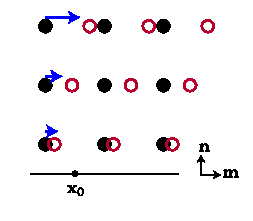
\includegraphics[scale=1.3]{figure/cinematica/scorrimento}
\end{center}

Since $\nabla\mathbf{u}=\gamma \mathbf{m} \otimes \mathbf{n}$, we deduce that
\begin{equation}
	\mathbf{E}=\frac{\gamma}{2}(\mathbf{m} \otimes \mathbf{n} +\mathbf{n} \otimes \mathbf{m}), \qquad \mathbf{W}=\frac{\gamma}{2}(\mathbf{m} \otimes \mathbf{n}-\mathbf{m} \otimes \mathbf{n}).
\end{equation}
Using \eqref{E12}, we immediately deduce that
\begin{equation}
	\frac{\delta\alpha}{2}=\mathbf{E} \mathbf{m} \cdot\mathbf{n}=\frac{\gamma}{2},
\end{equation}
and thus the shear coefficient $\gamma$ is equal to the change in angle between $\mathbf{m}$ and $\mathbf{n}$. For convenience, let us fix $\mathbf{x}_0=\mathbf{0}$, $\mathbf{m} =\mathbf{e}_1$ and $\mathbf{n}=\mathbf{e}_2$. Then, the representative matrices for $\mathbf{E}$ and $\mathbf{W}$ are:
\begin{equation}
	[\mathbf{E}(\mathbf{u})]=\frac{\gamma}{2}\begin{bmatrix}0&1&0\\1&0&0\\0&0&0\end{bmatrix}\quad\mathrm{and}\quad[\mathbf{W}(\mathbf{u})]=\frac{\gamma}{2}\begin{bmatrix}0&1&0\\-1&0&0\\0&0&0\end{bmatrix}.
\end{equation}
Since $\mathbf{u} (\mathbf{x})=\mathbf{E} \mathbf{x} +\mathbf{W} \mathbf{x}$, we conclude that
\begin{equation}
	\mathbf{u}(\mathbf{x})=\underbrace{\frac{\gamma}{2}(x_2 \mathbf{e}_1+x_1 \mathbf{e}_2)}_{\text{pure shear}} +\underbrace{ \frac{\gamma}{2}(x_2 \mathbf{e}_1-x_1 \mathbf{e}_2)}_{\text{infinitesimal rotation}}.
\end{equation}
Thus, the total displacement can be viewed as the sum of pure shear (given by $\mathbf{E} \mathbf{x}$) and an infinitesimal rotation (given by $\mathbf{W} \mathbf{x}$).  

\begin{center}
	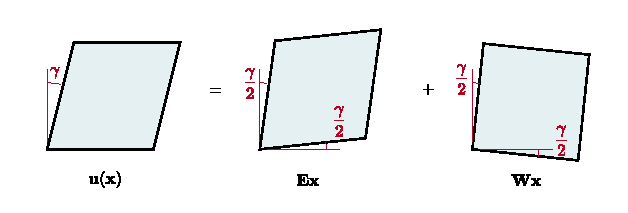
\includegraphics[scale=1.3]{figure/cinematica/scorrimento1}
\end{center}

In light of observation \ref{skvec}, the axis of $\mathbf{W}$ is
\begin{equation}
	\mathbf{w} =-\frac{\gamma}{2}\, \mathbf{e}_3.
\end{equation}
Thus, it is a rotation around the axis $\mathbf{e}_3$, by an angle $\gamma/2$; the negative sign indicates that the rotation is clockwise.

\begin{exercise}
	Given the displacement field
	\begin{equation}
		\mathbf{u}(\mathbf{x})=(\alpha_1 x_1x_2+\alpha_2 x_2)\mathbf{e}_1+(\beta_1 x_2+\beta_2 x_1)\mathbf{e}_2, \qquad \alpha_1, \alpha_2, \beta_1, \beta_2\in \mathbb{R},
	\end{equation}
	determine:
	\begin{enumerate}
		\item The deformed boundary of a square with side $L$ and two sides along the $x_1, x_2$ axes;
		\item 	The infinitesimal strain tensor and the infinitesimal rotation tensor;
		\item The final configuration and the change in length (using infinitesimal theory) of the diagonal inclined at $\pi/4$ with respect to $x_1$;
		\item The change in area (using infinitesimal theory) of the square introduced in point a).
	\end{enumerate}
	
	\begin{svolgimento}
		\begin{enumerate}
			\item Referring to the notation in the figure,
			\begin{center}
				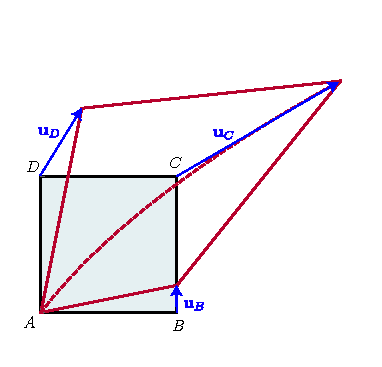
\includegraphics[scale=1]{figure/cinematica/esempio3d_1}
			\end{center}
			we can immediately calculate the displacement of the vertices:
			\begin{equation}
				\mathbf{u}_A=\mathbf{0}, \qquad \mathbf{u}_B=\beta_2 L \mathbf{e}_2, \qquad \mathbf{u}_C=(\alpha_1^2L+\alpha_2L)\mathbf{e}_1+(\beta_1+\beta_2)L\mathbf{e}_2, \qquad \mathbf{u}_D=\alpha_2L \mathbf{e}_1+\beta_1 L \mathbf{e}_2.
			\end{equation}
			The points on the side  $AB=\{ \mathbf{x}\in \mathcal{V} \,:\, \mathbf{x} =x_1\mathbf{e}_1, 0<x_1<L\}$ undergo the deformation
			\begin{equation}
				\mathbf{f}(\mathbf{x})=x_1\mathbf{e}_1+(x_2+\beta_2 x_1)\mathbf{e}_2,
			\end{equation}
			and thus the side $AB$ deforms into an inclined line at an angle given by
			\begin{equation}
				\delta x_2=\beta_2 x_1.
			\end{equation}
			\item The strain tensor is computed in the usual manner:
			\begin{equation}
				\mathbf{E}=\frac{1}{2}\left(\nabla \mathbf{u}+ (\nabla \mathbf{u})^{\top} \right)=
				\frac{1}{2}\begin{bmatrix} \alpha_1 x_2+ \alpha_2 & \alpha_1 x_1 +\beta_1 & 0\\
					\alpha_1 x_1+\beta_1 & \beta_2 & 0\\
					0 & 0 & 0 \end{bmatrix}.
			\end{equation}
		\end{enumerate}
	\end{svolgimento}
\end{exercise}

\begin{exercise}
	A \textit{strain gauge rosette} is an electromechanical device that measures the percentage elongation in three directions. By mounting such a device on the surface of a structure, it is possible to determine the axial strains in certain directions. A schematic representation of a rosette is shown in the figure. Assume that in an experiment, the specific elongations in the directions defined by the unit vectors $\ab$, $\bb$, and $\cb$ were measured, resulting in $\varepsilon_a$, $\varepsilon_b$, and $\varepsilon_c$. Using infinitesimal theory, determine the components of the specific elongation in the directions $\eb_1$ and $\eb_2$ and the angle change between $\eb_1$ and $\eb_2$.
	%
	\begin{center}
		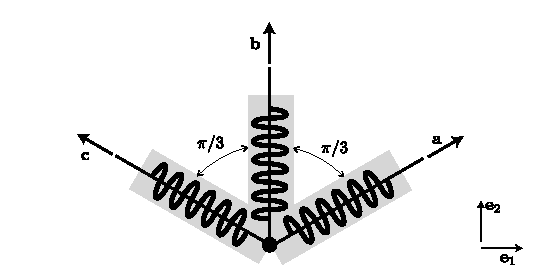
\includegraphics[scale=1.2]{figure/cinematica/rosetta.pdf}
	\end{center}
	
	\begin{svolgimento}
		Let us denote by
		\begin{equation}
			\ab = \frac{\sqrt{3}}{2}\eb_{1} + \frac12 \eb_2, \qquad \bb=\eb_2, \qquad \cb = -\frac{\sqrt{3}}{2}\eb_{1} + \frac12 \eb_2
		\end{equation}
		the unit vectors defining the three directions of the rosette. We need to solve the system
		\begin{equation}
			\begin{cases}
				\Eb \ab \cdot \ab = \dfrac{1}{2}(3 E_{11} + 2\sqrt{3} E_{12} + E_{22}) = \varepsilon_a,\\[.2cm]
				\Eb \bb \cdot \bb = E_{22} = \varepsilon_b,\\[.2cm]
				\Eb \cb \cdot \cb = \dfrac14 (3E_{11} - 2\sqrt{3}E_{12} + E_{22}) = \varepsilon_c,
			\end{cases}
		\end{equation}
		for the unknowns $E_{11}$, $E_{12}$, and $E_{22}$. The solution is
		\begin{equation}
			E_{11} = \frac13(2\varepsilon_a - \varepsilon_b + 2\varepsilon_c), \qquad E_{12} = \frac{\varepsilon_a - \varepsilon_c}{\sqrt{3}}, \qquad 
			E_{22} = \varepsilon_b.
		\end{equation}
	\end{svolgimento}
	
\end{exercise}

\begin{exercise}\label{defmedia}
	Let $\bar\Eb$ be the average strain of a configuration ${\Omega}$:
	\begin{equation}
		\bar{\Eb} = \frac{1}{\textrm{vol}({\Omega})}\int_{\Omega}\Eb.
	\end{equation}
	Prove that the average strain depends only on the displacement $\ub$ on the boundary and, in particular,
	\begin{equation}
		\bar{\Eb} = \frac{1}{2\textrm{vol}(\Omega)}\int_{\partial{\Omega}} \ub \otimes \nb + \nb \otimes \ub
	\end{equation}
	where $\textrm{vol}(\Omega)$ is the volume of $\Omega$ and $\nb$ is the normal to the boundary of ${\Omega}$.
	
	\begin{svolgimento}
		We use the following version of the divergence theorem (see \eqref{theodiv}):
		\begin{equation}
			\int_{\Omega} \nabla \varphi = \int_{\partial\Omega} \varphi \nb,
		\end{equation}
		where $\varphi$ is a scalar field. Choose $\varphi = \ub \cdot \ab$, with $\ab \in \Vc$ constant. We have
		\begin{equation}
			(\nabla \varphi)_i = \varphi,_i \eb_i = (\ub,_{i}\cdot \ab) \eb_i = (\eb_i \otimes \ub,_i) \ab = \nabla \ub^\top \, \ab.
		\end{equation}
		Therefore,
		\begin{equation}
			\left( \int_{\Omega} \nabla \ub^\top \right) \ab = \int_{\partial{\Omega}} (\ub \cdot \ab) \nb = \int_{\partial{\Omega}} (\nb \otimes \ub) \ab,
		\end{equation}
		from which we conclude that
		\begin{equation}
			\int_{\Omega} \nabla \ub^\top = \int_{\partial{\Omega}} \nb \otimes \ub.
		\end{equation}
		Given the definition of $\Eb$, it is then immediate to conclude that
		\begin{equation}
			\bar{\Eb} = \frac{1}{2 \operatorname{vol}(\Omega)} \int_{\partial{\Omega}} \ub \otimes \nb + \nb \otimes \ub.
		\end{equation}
	\end{svolgimento}
\end{exercise}

\begin{exercise}
	\item Consider a disk of radius $R$ centered at the origin of the Cartesian coordinate system $\{O; x_1, x_2\}$. On the boundary of the disk, the displacement is imposed as
	\begin{equation}
		\ub(\xb) = (\alpha \eb_1 \otimes \eb_1 + \beta \eb_2 \otimes \eb_1) \xb \qquad \alpha, \beta \in \Ro.
	\end{equation}
	Determine the average strain of the disk.
	\begin{svolgimento}
		Given the geometry, it is convenient to use polar coordinates, so that the position of a generic point on the disk is
		\begin{equation}
			\xb = \rho \cos\vartheta \eb_1 + \rho \sin\vartheta \eb_2, \qquad 0 \leq \rho < R, \quad 0 \leq \vartheta < 2\pi.
		\end{equation}
		The unit normal vector to the disk is 
		\begin{equation}
			\nb = \cos\vartheta \eb_1 + \sin\vartheta \eb_2.
		\end{equation}
		With the aim of using the result from exercise \ref{defmedia}, we determine
		\begin{equation}
			\begin{aligned}
				\frac12 (\ub \otimes \nb + \nb \otimes \ub) &= \alpha R \cos^2 \vartheta \eb_1 \otimes \eb_1 + \frac{1}{2} R \cos\vartheta (\alpha \sin\vartheta + \beta \cos\vartheta) (\eb_1 \otimes \eb_2 + \eb_2 \otimes \eb_1)\\
				&+ R \beta \sin\vartheta \cos\vartheta\, \eb_2 \otimes \eb_2,
			\end{aligned}
		\end{equation}
		from which we get
		\begin{equation}
			\bar{\Eb} = \frac{1}{\pi R^2} \int_0^{2\pi} \frac12 (\ub \otimes \nb + \nb \otimes \ub) R \, d\vartheta = \alpha \eb_1 \otimes \eb_1 + \frac \beta 2 (\eb_1 \otimes \eb_2 + \eb_2 \otimes \eb_1).
		\end{equation}
	\end{svolgimento}
\end{exercise}

\begin{exercise}
	Let  $\ub: \Omega \to \Vc$ be a displacement field tangential to the boundary of $\Omega$. Show that in infinitesimal theory, the specific volume change is, on average, zero.
	\begin{svolgimento}
		Using the result from exercise \ref{defmedia}, we can determine the average specific volume change:
		\begin{equation}
			\operatorname{tr} \bar{\Eb} = \frac{1}{\operatorname{vol}(\Omega)} \int_{\partial{\Omega}} \ub \cdot \nb = 0
		\end{equation}
		since $\ub \cdot \nb = 0$ on $\partial{\Omega}$, as $\ub$ is tangential to the boundary of $\Omega$.
	\end{svolgimento}
\end{exercise}


\section{The Compatibility Condition}

Given an arbitrary deformation field \(\Eb\), the relationship between displacement and deformation
\begin{equation}
	\Eb = \frac{1}{2} (\nabla \ub + \nabla \ub^\top)
\end{equation}
constitutes a first-order linear differential equation in the displacement field \(\ub\), whose solution is not guaranteed to exist. We will show that a \textit{necessary} condition for the existence of solutions is that the deformation field satisfies a certain compatibility condition, which is also \textit{sufficient} to guarantee existence if the domain is simply connected.

First, note that the deformation field \(\Eb\) and the infinitesimal rotation vector \(\wb\) satisfy the following condition:
\begin{equation}\label{RotE}
	\Curl \Eb = \nabla \wb.
\end{equation}
% Recall that the components of the curl of a vector \(\vb\) are 
%\begin{equation}
%(\Curl \vb)_i = \epsilon_{ijk} v_{k,j}
%\end{equation}
% where
%\begin{equation}
%\epsilon_{ijk} = \eb_i \times \eb_j \cdot \eb_k
%\end{equation}
% is the Ricci symbol (see \eqref{Ricci}).
%, such that
%\begin{equation}
%\epsilon_{ijk} = \begin{cases} +1 & \text{if all indices \(i, j, k\) are different and their sequence} \\ & \text{is an even permutation of \(1, 2, 3\)}; \\ 0 & \text{if at least two of the indices \(i, j, k\) are equal;} \\ -1 & \text{if all indices \(i, j, k\) are different and their sequence} \\ & \text{is an odd permutation of \(1, 2, 3\)}. \end{cases}
%\end{equation}
% Given a tensor field \(\Ab\), its curl is defined as:
%\begin{equation}
%(\Curl \Ab) \ab \coloneqq \Curl(\Ab^\top \ab), \qquad \forall \ab \in \Vc;
%\end{equation}
% in components:
%\begin{equation}
%	(\Curl \Ab)_{ij} = \epsilon_{ipq} A_{jq},_{p}.
%\end{equation}
To prove \eqref{RotE}, we calculate the curl of the gradient of the displacement (see \eqref{RotT}):
\begin{equation}
	(\Curl(\nabla \ub))_{ij} = \epsilon_{ipq} (\nabla \ub)_{jq,p} = \epsilon_{ipq} (u_{j,q})_p = \epsilon_{ipq} u_{j,qp} = 0;
\end{equation}
furthermore, we have
\begin{equation}
	(\Curl(\nabla \ub^\top))_{ij} = \epsilon_{ipq} (u_{q,j}),_p = \epsilon_{ipq} u_{q,jp} = (\epsilon_{ipq} u_{q,p}),_j = 2 w_{i,j} = 2 (\nabla \wb)_{ij}.
\end{equation}
In the last equality, we introduced the vector
\begin{equation}
	\wb \coloneqq \frac{1}{2} \Curl \ub;
\end{equation}
since, using \eqref{epsdel}, we can write the following sequence of equalities:
\begin{equation}
	\begin{aligned}
		(\wb \times \ab)_i &= \epsilon_{ijk} w_j a_k = \frac{1}{2} \epsilon_{ijk} \epsilon_{jpq} u_{q,p} a_k \\
		&= -\frac{1}{2} \epsilon_{jik} \epsilon_{jpq} u_{q,p} a_k = -\frac{1}{2} (\delta_{ip} \delta_{kq} - \delta_{iq} \delta_{kp}) u_{q,p} a_k \\
		&= \frac{1}{2} (u_{i,k} - u_{k,i}) a_k = \frac{1}{2} (\nabla \ub - \nabla \ub^\top)_{ik} a_k = W_{ik} a_k = (\Wb \ab)_i,
	\end{aligned}
\end{equation}
for every \(\ab\), we can identify \(\wb\) with the axial part of the infinitesimal rotation tensor \(\Wb\), so that
\begin{equation}
	\Wb \ab = \frac{1}{2} \Curl \ub \times \ab.
\end{equation}

We then conclude that
\begin{equation}
	\Curl \Eb = \frac{1}{2} \big( \Curl (\nabla \ub) + \Curl (\nabla \ub^\top) \big) = \nabla \wb.
\end{equation}
Applying the curl operator again to \eqref{RotE}, we conclude that a necessary condition for the existence of a displacement field is that \(\Eb\) satisfies the following \textit{compatibility condition}:
\begin{definition}
	\begin{equation}\label{RotRot}
		\Curl \Curl \Eb = \mathbf{0}.
	\end{equation}
\end{definition}

We now prove that the condition \eqref{RotRot} is not only sufficient but also necessary, if the domain is simply connected; in other words, if \(\Curl \Curl \Eb = \mathbf{0}\), then there certainly exists a vector field \(\ub\) such that \(\Eb = \sym \nabla \ub\).

To prove this, we need two preparatory results:
\begin{enumerate}
	\item Let \(\Tb \in \Lin\) such that \(\Curl \Tb = \mathbf{0}\), then there exists a vector field \(\ub\) such that\footnote{To prove this, consider the vectors
		\begin{equation}
			\ab_i = \Tb^\top \eb_i,
		\end{equation}
		where \(\eb_i\) are the basis vectors; we have that
		\begin{equation}
			\Curl \ab_i = \Curl (\Tb^\top \eb_i) = \Curl(\Tb^\top) \eb_i = 0
		\end{equation}
		and thus there exist scalar fields \(u_i\) such that \(\ab_i = \nabla u_i\).
		%
		Define \(\ub \coloneqq u_i \eb_i\); then
		\begin{equation}
			\ab_i = \nabla u_i = \nabla(\ub \cdot \eb_i) = (\nabla \ub)^\top \eb_i = \Tb^\top \eb_i,
		\end{equation}
		which gives \eqref{Tnabu}.}
	\begin{equation}\label{Tnabu}
		\Tb = \nabla \ub.
	\end{equation}
	\item Let \(\Tb \in \Lin\) such that \(\Curl \Tb = \mathbf{0}\) and \(\operatorname{tr} \Tb = 0\), then there exists \(\Wb \in \Skw\) such that\footnote{
		To prove this: let \(\ub\) be the vector defined in the previous note and \(\Wb\) the skew-symmetric tensor associated with \(-\ub\). Then
		\begin{equation}
			\Div \ub = \operatorname{tr} \nabla \ub = \operatorname{tr} \Tb = 0.
		\end{equation}
		By \eqref{identitadiff}$_9$
		\begin{equation}
			-\Curl \Wb = (\Div \ub)\Ib - \nabla \ub = -\nabla \ub = -\Tb,
		\end{equation}
		which gives the result.
	}
	\begin{equation}
		\Tb = \Curl \Wb.
	\end{equation}
\end{enumerate}

Now, let's return to proving that if \(\Curl \Curl \Eb = \mathbf{0}\), then there exists a vector field \(\ub\) such that \(\Eb = \sym \nabla \ub\). Assume that \(\Curl \Curl \Eb = \mathbf{0}\) in \(\Omega\). Let \(\Ab = \Curl \Eb\); since \(\Eb \in \Sym\),
\eqref{identitadiff}$_8$ implies that
\begin{equation}
	\operatorname{tr} \Ab = 0.
\end{equation}
Since \(\Curl \Ab = \mathbf{0}\), there exists a tensor field \(\Wb \in \Skw\) such that
\begin{equation}
	\Ab = -\Curl \Wb.
\end{equation}
Since \(\Ab = \Curl \Eb\),
\begin{equation}
	\Curl (\Eb + \Wb) = \mathbf{0};
\end{equation}
therefore, there exists a vector field \(\ub\) such that
\begin{equation}
	\Eb + \Wb = \nabla \ub.
\end{equation}
Taking the symmetric part of the last equality, we conclude that there exists \(\ub\) such that
\begin{equation}
	\Eb = \sym \nabla \ub.
\end{equation}


